% Preamble
\documentclass{article}


% Packages
\usepackage[legalpaper, portrati, margin=0.9in]{geometry}
\usepackage{amsmath}
\usepackage{bm}
\usepackage{amssymb}
\usepackage{gensymb}
\usepackage{mathtools}
\usepackage{xcolor}
\usepackage{caption}
\usepackage{subcaption}
\usepackage{pgfplots}
\pgfplotsset{compat=1.17}
\usepackage{tikz}
\usepackage{tkz-euclide}


% Macros
\DeclarePairedDelimiter\ceil{\lceil}{\rceil}
\DeclarePairedDelimiter\floor{\lfloor}{\rfloor}

\newcommand*{\longunderscore}
{
    \rule{0.25cm}{0.15mm}
}


% File info
\title{Algebra Notes}
\author{Eric Xia}
\date{Last Updated 21 August 2020}


% Document
\begin{document}

    \maketitle
    \tableofcontents
    \pagebreak

    \section{Introduction to Calculus}

    \subsection{Limits}
        \color{purple} \textbf{The Epsilon-Delta ($\epsilon-\delta$) Definition of Limits:}
        \color{black} \\

        \noindent Let $f$ be a real-valued function, defined around around $a$.
        Then the \textbf{limit}, $L$, as $f(x)$ approaches $a$, or \textbf{converges} to $a$, is \\

        \begin{equation*}
            \lim_{x \to a} f(x) = L
        \end{equation*}

        \noindent If, $\forall \epsilon > 0$, there exists $\delta > 0$ such that if $x$ is
        within $\delta$ of $a$ (with $x\not = a$), then $f(x)$ is within $\epsilon$ of $L$.
        In other words, \\

        \begin{equation*}
            \text{If } 0 < |x-a| < \delta, \text{ then } |f(x)-L| < \epsilon
        \end{equation*}

        \begin{figure} [hbt!]
            \centering
            \begin{subfigure}[b]{.45\textwidth}
                \includegraphics{Resources/Unit1Limits/limit1.PNG}
            \end{subfigure}
            \begin{subfigure}[b]{.45\textwidth}
                \includegraphics{Resources/Unit1Limits/limit2.PNG}
            \end{subfigure}
        \end{figure}

        \noindent It is easiest to think of the limit of a function at a certain point, $a$,
        as the value of the function near $a$. For a limit, $L$, to exist at $a$, the
        \textbf{right-hand limit ($a^+$)} and the \textbf{left-hand limit ($a^-$)} must be equal. \\

        \begin{equation*}
            \lim_{x \to a} f(x) = L \implies \lim_{x \to a^+} f(x) = L = \lim_{x \to a^-} f(x)
        \end{equation*}

        \noindent \color{blue} \textit{Example 1: Find $\lim_{x\to 4}f(x)$, where the function
        $f(x)$ is given by the graph}. \color{black} \\

        \begin{center}
            \begin{tikzpicture}
                \begin{axis}[
                    axis lines = center,
                    axis equal image,
                    xmin = -3,
                    xmax = 7,
                    ymin = -3,
                    ymax = 7,
                ]
                %f(x)
                \addplot [
                    samples = 200,
                    color = red,
                ]
                {(x-2)^2-1};
                \addlegendentry{$f(x)$}
                \end{axis}
            \end{tikzpicture}
        \end{center}

        \begin{equation*}
            \lim_{x\to4^+}f(x) = 2 = \lim_{x\to4^-} f(x) \\
        \end{equation*}
        \begin{equation*}
            \therefore \lim_{x\to4} f(x) = 2
        \end{equation*}

        \noindent \color{blue} \textit{Example 2: Determine $\lim_{x\to 1} g(x)$, where the
        function $g(x)$ is graphed below. It is given that $g(x)$ is defined for all real numbers
        except $x=1$ and the graph of $g(x)$ is divided by the asymptote $x=1$.} \color{black} \\

        \begin{center}
            \begin{tikzpicture} [scale=0.75]
                \begin{axis}[
                    axis lines = center,
                    xmin = -20,
                    xmax = 20,
                    ymin = -20,
                    ymax = 20
                ]
                %g(x)
                \addplot [
                    unbounded coords=jump,
                    domain=-20:-2,
                    samples=41,
                    color=blue
                ]
                {(3*x+6)/(x-1)};
                \addlegendentry{$g(x)$}
                \addplot [unbounded coords=jump,
                    domain=-2:1,
                    samples=16,
                    color=blue,
                ]
                {(3*x+6)/(x-1)};
                \addplot [unbounded coords=jump,
                    domain=1:20,
                    samples=46,
                    color=blue,
                ]
                {(3*x+6)/(x-1)};
                %Vertical Asymptote
                \draw[dashed] (1,\pgfkeysvalueof{/pgfplots/ymin}) --
                (1,\pgfkeysvalueof{/pgfplots/ymax})
                (\pgfkeysvalueof{/pgfplots/xmin},3) --
                (\pgfkeysvalueof{/pgfplots/xmax},3);
                \end{axis}
            \end{tikzpicture}
        \end{center}

        \begin{equation*}
            \lim_{x\to 1^+}g(x) = \infty
        \end{equation*}
        \noindent and
        \begin{equation*}
            \lim_{x\to 1^-}g(x) = -\infty
        \end{equation*}

        \noindent Since the right-hand and left-hand limits do not equal each other,
        $\lim_{x\to1}g(x)$ does not exist.



    \subsection{Limit Properties}
        Assume $\lim_{x\to a}f(x)$ and $\lim_{x\to a}g(x)$ exist and that $c$ is any constant.
        Then the following properties hold true. \\

        \begin{center}
            \begin{tabular}{|c|c|}
                \hline
                $\lim_{x\to a} c=c$ & \textbf{Limit of a Constant} \\
                \hline
                $\lim_{x\to a} [cf(x)]=c\lim_{x\to a} f(x)$ & \textbf{Constant Multiple} \\
                \hline
                $\lim_{x\to a} [f(x)\pm g(x)=\lim_{x\to a}f(x)\pm\lim_{x\to a} g(x)]$ & \textbf{Sum/Difference} \\
                \hline
                $\lim{x\to a}[f(x)g(x)]=\lim_{x\to a}f(x)\lim_{x\to a}g(x)$ & \textbf{Product} \\
                \hline
                $\lim_{x\to c}(f(g(x)))=f\left(\lim_{x\to c}g(x)\right)$ &
                \textbf{Composition} \\
                \hline
                $\lim_{x\to a} \left[\frac{f(x)}{g(x)}\right]=\frac{\lim_{x\to a}f(x)}{\lim_{x\to a}g(x)}, \lim_{x\to a}g(x)\not = 0$. & \textbf{Quotient} \\
                \hline
                $\lim_{x\to a}[f(x)]^n=\left[\lim_{x\to a}f(x)\right]^n, n\in \mathbb{R}$ & \textbf{Exponent} \\
                \hline
                $\lim_{x\to a}\sqrt[3]{f(x)}\sqrt[n]{\lim_{x\to a}[f(x)]}$ & \textbf{Root} \\ \hline
                $\lim_{x\to a}x=a$ & \textbf{Limit of a Variable} \\
                \hline
            \end{tabular}
        \end{center}



    \subsection{Finding Limits from Tables}
        Tables should always be the last resort when attempting to determine limits, because
        of their tendency to be tedious. \\

        \noindent \color{blue} \textit{Example: The function $g$ is defined over the real numbers.
        This table gives a few values of $g$ What is a reasonable estimate for $\lim_{x\to 4}g(x)$?}
        \color{black} \\

        \begin{tabular}{ccccccc}
            $x$ & 3.9 & 3.99 & 3.999 & 4.001 & 4.01 & 4.1 \\
            \hline
            $g(x)$ & 11.21 & 11.92 & 11.99 & 12.01 & 12.08 & 12.81
        \end{tabular}

        \noindent $lim_{x\to 4}g(x)$ represents the limit of $g$ as $x$ approaches
        4. Looking over the table, we see that the left-hand limit appears to approach 12 as
        $x$ gets progressively larger. \\

        \begin{tabular}{cccc}
            $x$ & 3.9 & 3.99 & 3.999 \\
            \hline
            $g(x)$ & 11.21 & 11.92 & 11.99
        \end{tabular}

        \noindent We also see that the right-hand limit appears to approach 12 as $x$ gets
        progressively smaller. \\

        \begin{tabular}{cccc}
            $x$ & 4.001 & 4.01 & 4.1 \\
            \hline
            $g(x)$ & 12.01 & 12.08 & 12.81
        \end{tabular}

        \noindent Since the right-hand and left-hand limits are equal, we can conclude
        that $\lim_{x\to 4}g(x)=12$.



    \subsection{Evaluating Limits Algebraically}
        \color{purple} \textbf{The 3 Main Algebraic Limit Strategies:} \color{black} \\
        \noindent \color{purple} \textbf{1. Factoring} \color{blue} \\
        \textit{Example: Determine the limit} \color{black} \\

        \begin{align*}
            \lim_{x\to -1}\frac{x^2-x-2}{x^2-2x-3} &= \lim_{x\to -1}\frac{(x+1)(x-2)}{(x+1)(x-3)} \\
            &= \lim_{x\to -1}\frac{x-2}{x-3} \\
            &= \frac{-1-2}{-1-3} \\
            &= \frac{3}{4}
        \end{align*}

        \noindent \color{purple} \textbf{2. Conjugates} \color{blue} \\
        \textit{Example: Determine the limit} \color{black} \\
        \begin{align*}
            \lim_{x\to 4}\frac{\sqrt{x}-2}{x-4}
            &= \lim_{x\to 4}\frac{\sqrt{x}-2}{x-4}\cdot\frac{\sqrt{x}+2}{\sqrt{x}+2} \\
            &= \lim_{x\to 4}\frac{1}{\sqrt{x}+2} \\
            &= \frac{1}{4}
        \end{align*}

        \pagebreak
        \noindent \color{purple} \textbf{3. Trig Identities} \color{blue} \\
        \textit{Example: Determine the limit} \color{black} \\
        \begin{align*}
            \lim_{x\to 0} \frac{\sin{(x)}}{\sin{(2x)}}
            &= \lim_{x\to 0} \frac{\sin{(x)}}{2\sin{(x)}\cos{(x)}} \\
            &= \lim_{x\to 0} \frac{1}{2\cos{(x)}} \\
            &= \frac{1}{2}
        \end{align*}



    \subsection{Asymptotes}
        \color{purple} \textbf{Horizontal Asymptotes:} \color{black} \\
        \noindent The line $y=b$ is a \textit{horizontal asymptote} of the graph of $y=f(x)$ if \\

        \begin{equation*}
            \lim_{x\to\infty}f(x)=b\text{ or }\lim_{x\to-\infty}f(x)=b
        \end{equation*}

        \noindent It is important to note that horizontal and slant asymptotes \textit{can} be crossed,
        as they describe the general behavior of the functions as they near the edges of the graph.
        On the other hand, vertical asymptotes cannot be crossed as they describe particular
        behavior of the function itself, rather than the edges of the graph. Below is an example
        of a horizontal asymptote being crossed. \\

        \begin{center}
            \begin{tikzpicture}
                \begin{axis}[
                    axis lines = center,
                    xmin = -10,
                    xmax = 15,
                    ymin = -3,
                    ymax = 6,
                    xlabel={$x$},
                    ylabel={$y$},
                ]
                %f(x)
                \addplot [
                    domain=-10:15,
                    samples=100,
                    color=red
                ]
                {(3*x^2-8*x+7)/(x^2-4*x+5)};
                \addlegendentry{$f(x)=\frac{3x^2-8x+7}{x^2-4x+5}$}
                %asymptote
                \draw[
                    dashed
                ]
                (-10,3) -- (15,3);
                \end{axis}
            \end{tikzpicture}
        \end{center}

        \noindent \color{purple} \textbf{Vertical Asymptotes:} \color{black} \\
        The line $x=a$ is a \textit{vertical asymptote} of the graph of $y=f(x)$ if at least one
        of the below expressions holds. \\

        \begin{equation*}
            \lim_{x\to a^-}f(x)=\pm\infty,
            \lim_{x\to a^+}f(x)=\pm\infty
        \end{equation*}

        \noindent Example of a graph containing a vertical asymptote: \\

        \begin{center}
            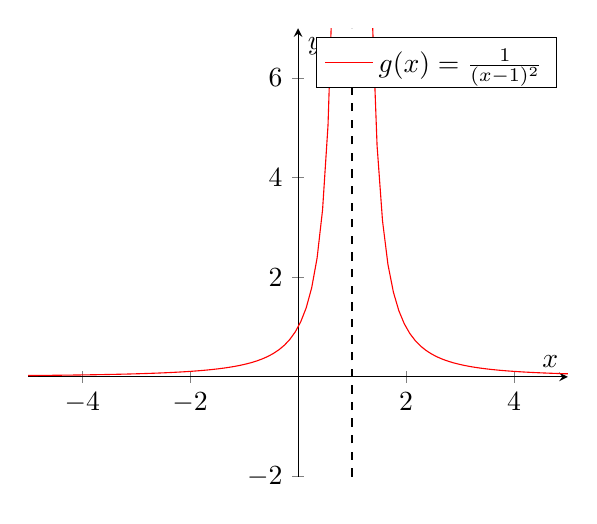
\begin{tikzpicture}
                \begin{axis}[
                    axis lines = center,
                    xmin = -5,
                    xmax = 5,
                    ymin = -2,
                    ymax = 7,
                    xlabel={$x$},
                    ylabel={$y$},
                ]
                %g(x)
                \addplot [
                    domain=-5:5,
                    samples=100,
                    color=red
                ]
                {(1)/((x-1)^2)};
                \addlegendentry{$g(x)=\frac{1}{(x-1)^2}$}
                %asymptote
                \draw[
                    dashed
                ]
                (1,-2) -- (1,7);
                \end{axis}
            \end{tikzpicture}
        \end{center}

        \noindent \color{purple} \textbf{The Rational Function Theorem:} \color{black} \\
        \noindent When $\lim_{x\to\pm\infty}\frac{P(x)}{Q(x)}=0$, $y=0$ is a horizontal asymptote
        of the graph of $y=\frac{P(x)}{Q(s)}$. \\
        When $\lim_{x\to\pm\infty}\frac{P(x)}{Q(x)}=\pm\infty$, the graph of $y=\frac{P(x)}{Q(x)}$
        has no horizontal asymptotes. \\
        When $\lim_{x\to\pm\infty}\frac{P(x)}{Q(x)}=\frac{a_n}{b_n}$, $y=\frac{a_n}{b_n}$ is a
        horizontal asymptote of the graph of $y=\frac{P(x)}{Q(x)}$.

    \pagebreak
    \subsection{The Squeeze Theorem}
        Functions $g$ and $h$ are strategically chosen to satisfy the conditions outlined in the
        definition. Notice how, in the figure after the definition, function $f$ is being
        "squeezed" between functions $g$ and $h$, hence the name. \\

        \noindent \color{purple} \textbf{The Squeeze Theorem:} \color{black} \\
        Assume that functions $f,g,h$ defined n $D\subseteq\mathbb{R}$ satisfy \\

        \begin{equation*}
            g(x)\leq f(x)\leq h(x),\forall x\in D
        \end{equation*}

        \noindent If $\lim_{x\to a}g(x)=\lim_{x\to a}h(x)=L$, then $\lim_{x\to a}f(x)=L$. \\

        \begin{center}
            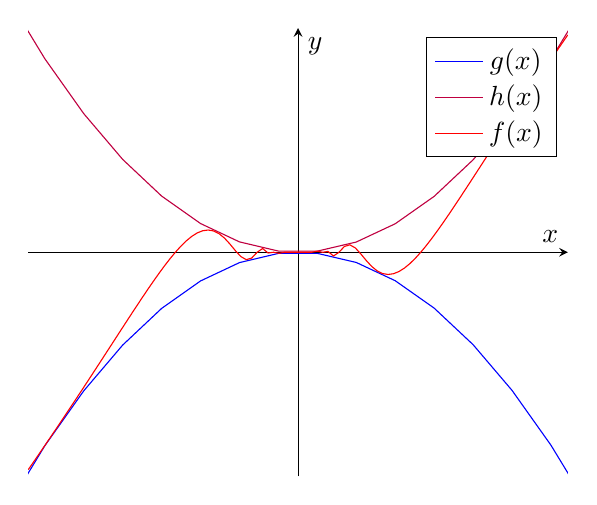
\begin{tikzpicture}
                \begin{axis}[
                    axis lines = center,
                    xmin = -0.7,
                    xmax = 0.7,
                    ymin = -0.5,
                    ymax = 0.5,
                    xlabel={$x$},
                    ylabel={$y$},
                    \pgfplotset{ticks=none}
                ]
                    %g(x)
                    \addplot [
                        samples=100,
                        color=blue
                    ]
                    {-x^2};
                    \addlegendentry{$g(x)$}
                    %h(x)
                    \addplot[
                        samples=100,
                        color=purple
                    ]
                    {x^2};
                    \addlegendentry{$h(x)$}
                    %f(x)
                    \addplot[
                        domain=-0.7:0.7,
                        samples=100,
                        color=red
                    ]
                    {x^2*sin(deg(1/\x))};
                    \addlegendentry{$f(x)$}
                \end{axis}
            \end{tikzpicture}
        \end{center}

        \noindent \color{blue}
        \textit{Example 1: Given an infinite sequence $\{a_n\}$ that satisfies
        $\frac{2n^2-7}{4n+5}<a_n<\frac{3n^2+8}{6n-1}$ for all positive integers $n$, evaluate} \\

        \begin{equation}
            \lim_{n\to \infty}\frac{3na_n}{(n+1)^2}
        \end{equation}

        \color{black} \noindent We transform the middle term of the inequality to the desired
        expression through manipulating each side of the inequality. Then the inequality becomes \\

        \begin{equation*}
            \frac{3n}{(n+1)^2}\cdot\frac{2n^2-7}{4n+5}<\frac{3na_n}{(n+1)^2}<\frac{3n}{(n+1)^2}\cdot\frac{3n^2+8}{6n-1}
        \end{equation*}

        \noindent Now we can take the limits of the top and bottom functions. \\

        \begin{align*}
            \lim_{n\to \infty}\frac{3n(2n^2-7)}{(4n+5)(n+1)^2} &= \frac{3}{2} \\
            \lim_{n\to\infty}\frac{3n(3n^2+8)}{(6n-1)(n+1)^2} &= \frac{3}{2}
        \end{align*}

        \noindent Since the top and bottom functions are equal, we can conclude that \\

        \begin{equation*}
            \lim_{n\to\infty} \frac{3na_n}{(n+1)^2}=\frac{3}{2}
        \end{equation*}

        \noindent \color{blue} \textit{Example 2: Evaluate the limit} \\

        \begin{equation*}
            \lim_{n\to\infty}\sqrt[n]{3^n+\{2|\sin{(n^n)}\}^n}
        \end{equation*}

        \color{black} \noindent We can note that \\

        \begin{equation*}
            0\leq|\sin{(n^n)}|\leq1
        \end{equation*}

        \noindent Then we can write \\

        \begin{equation*}
            \sqrt[n]{3^n}\leq\sqrt[n]{3^n+\{2|\sin{(n^n)}\}^n}\leq\sqrt[n]{3^n+2^n}\leq\sqrt[n]{2\cdot3^n}
        \end{equation*}

        \noindent The left side reduces to 3, whereas the right side becomes \\

        \begin{equation*}
            \lim_{n\to\infty}\sqrt[n]{2\cdot3^n} = 3\lim_{n\to\infty}\sqrt[n]{2}=3
        \end{equation*}

        \noindent Thus we can conclude that \\

        \begin{equation*}
            \lim_{n\to\infty} \sqrt[n]{3^n+\{2|\sin{(n^n)}|\}^n} = 3
        \end{equation*}

        \noindent \color{blue} \textit{Example 3: Evaluate the limit} \\
        \begin{equation*}
            \lim_{x\to\infty}\frac{\sin{x}}{x}
        \end{equation*} \color{black}

        \noindent Since $\forall x,-1\leq\sin{x}\leq1$, it follows that if $x>0$ then
        $-\frac{1}{x}\leq\frac{\sin{x}}{x}\leq\frac{1}{x}$. As $x\rightarrow\infty$,
        $-\frac{1}{x}$ and $\frac{1}{x}$ both approach 0. Therefore, by the Squeeze Theorem,
        $\frac{\sin{x}}{x}$ also approaches 0. \\



    \subsection{Limit of a Quotient of Polynomials}
        For the function $f(x)=\frac{P(x)}{Q(x)}$, where $P(x)$ is a polynomial of degree $n$
        and $Q(x)$ is a polynomial of degree $m$, the following expressions hold. Let $a_n$
        and $b_n$ be the leading coefficients of $P(x)$ and $Q(x)$ respectively. Then \\

        \begin{equation*}
            \text{If $n>m$, then }\lim_{x\to\infty}f(x)=\infty\text{ and }
            \lim_{x\to-\infty}f(x)=-\infty
        \end{equation*}

        \begin{equation*}
            \text{If $n=m$, then }\lim_{x\to\pm\infty}f(x)=\frac{a_n}{b_m}
        \end{equation*}

        \begin{equation*}
            \text{If $n<m$, then }\lim_{x\to\pm\infty}f(x)=0
        \end{equation*}

        \noindent This method is a shortcut found through dividing each of the terms of $P(x)$
        and $Q(x)$ by the highest power of $x$ found in $f(x)$, then taking the individual limits
        of each separated term through basic limit properties. For example, see below. \\

        \noindent \color{blue} \textit{Example: Evaluate the limit} \color{black} \\

        \begin{align*}
            \lim_{x\to\infty}\frac{x^3-4x^2+7}{3-6x-2x^3} &=
            \lim_{x\to\infty}\frac{1-\frac{4}{x}+\frac{7}{x^3}}{\frac{3}{x^3}-\frac{6}{x^2}-2} \\
            &= \frac{\lim_{x\to\infty}(1)-\lim_{x\to\infty}\left(\frac{4}{x}\right)+\lim_{x\to\infty}\left(\frac{7}{x^3}\right)}{\lim_{x\to\infty\left(\frac{3}{x^3}\right)}-\lim_{x\to\infty}\left(\frac{6}{x^2}\right)-\lim_{x\to\infty}(2)} \\
            &= \frac{1-0+0}{0-0-2} \\
            &= -\frac{1}{2}
        \end{align*}

        \noindent Note that in this case, $n=m$, so $\frac{a_n}{b_n}\implies -\frac{1}{2}$.
        Since the properties described preceding this example can be observed in all quotients
        of polynomials, we can thus make generalizations as specificed above.



    \subsection{L'Hospital's Rule}
        \textbf{L'Hospital's} is a method of evaluating limits of indeterminate forms, learned
        after gaining knowledge of derivatives. \textbf{Indeterminate forms} are expressions i
        nvolving two functions whose limits cannot be determined solely from the limits of the
        individual functions. \\

        \noindent \color{purple} \textbf{The 7 Indeterminate Forms:} \\ \color{black}

        \begin{equation*}
            \frac{0}{0}, \frac{\infty}{\infty}, 0\cdot\infty, \infty-\infty, 0^0, 1^\infty, \infty^0
        \end{equation*}

        \noindent \color{purple} \textbf{L'Hospital's Rule:} \color{black} \\
        Suppose that we have either of the cases below \\

        \begin{equation*}
            \lim_{x\to a}\frac{f(x)}{g(x)}=\frac{0}{0}, \lim_{x\to a}\frac{f(x)}{g(x)}=\frac{\pm\infty}{\pm\infty}
        \end{equation*}

        \noindent where $a\in\mathbb{R}, \infty$ or $-\infty$. Then \\

        \begin{equation*}
            \lim_{x\to a}\frac{f(x)}{g(x)}=\lim_{x\to a}\frac{f'(x)}{g'(x)}
        \end{equation*}

        \noindent \color{blue} \textit{Example 1: Evaluate the limit} \\

        \begin{equation*}
            \lim_{t\to 1}\frac{5t^4-4t^2-1}{10-t-9t^3}
        \end{equation*}
        \color{black} We have an $\frac{0}{0}$ indeterminate form here, so we use L'Hospital's to get \\

        \begin{equation}
            \lim_{t\to 1}\frac{5t^4-4t^2-1}{10-t-9t^3}=\lim_{t\to 1}\frac{20t^3-8t}{-1-27t^2}
            =\frac{20-8}{-1-27}=-\frac{3}{7}
        \end{equation}

        \noindent \color{blue} \textit{Example 2: Evaluate the limit} \\

        \begin{equation*}
            \lim_{x\to-\infty}xe^x
        \end{equation*}
        \color{black} This expression is in the form $(\infty)(0)$, meaning we will have to write
        the expression as a quotient. We know that $\frac{1}{e^x}=e^{-x}$, so we can rewrite the
        limit as \\

        \begin{equation*}
            \lim_{x\to-\infty}xe^x=\lim_{x\to-\infty}\frac{x}{e^-x}=\lim_{x\to-\infty} \frac{1}{-e^-x}=0
        \end{equation*}

        \noindent \color{blue} \textit{Example 3: Evaluate the limit} \\

        \begin{equation*}
            \lim_{x\to\infty}x^{\frac{1}{x}}
        \end{equation*} \color{black}

        \noindent This limit is of the form $\infty^0$, so we have to rewrite this expression as a different
        limit. Let \\

        \begin{equation*}
            y &= x^{\frac{1}{x}} \\
        \end{equation*}

        \noindent Since \\

        \begin{equation*}
            e^{\ln{(y)}}=y
        \end{equation*}

        \noindent we can rewrite our limit as \\

        \begin{align*}
            \lim_{x\to\infty}x^{\frac{1}{x}} &= \lim_{x\to\infty} y \\
            &= \lim_{x\to\infty}e^{\ln{(y)}} \\
            &= e^{\lim_{x\to\infty}\ln{(y)}} \\
            &= e^0 \\
            &= 1
        \end{align*}

        \noindent L'Hospital's can help us prove \textbf{the basic trig limit}, useful for
        evaluating many trig limits. \\

        \begin{equation*}
            \lim_{\theta\to0}\frac{\sin{\theta}}{\theta}=1 \text{ if $\theta$ is measured in radians}
        \end{equation*}



    \pagebreak
    \subsection{Limit Strategies}
        KhanAcademy provides a convenient flowchart to illustrate a strategy to find limits: \\

        \begin{figure} [hbt!]
            \centering
            \includegraphics[scale=0.5]{Resources/Unit1Limits/limitstrat.png}
        \end{figure}

        \noindent \color{blue} \textit{Example 1:} \color{black} \\

        \begin{align*}
            \lim_{x\to 0}\frac{\sin{3x}}{x} &= \lim_{x\to0}\frac{3\sin{3x}}{3x} \\
            &= 3\lim_{x\to0}\frac{\sin{3x}}{3x} \\
            &= 3\cdot1\\
            &= 3
        \end{align*}

        \pagebreak
        \noindent \color{blue} \textit{Example 2:} \color{black} \\

        \begin{align*}
            \lim_{x\to0}\frac{\sin{2x}}{3x} &= \frac{1}{3}\lim_{x\to0}\frac{\sin{2x}}{x}\cdot\frac{2}{2} \\
            &= \frac{2}{3}\lim_{x\to0}\frac{\sin{2x}}{2x} \\
            &=\frac{2}{3}
        \end{align*}

        \noindent \color{blue} \textit{Example 3:} \color{black} \\

        \begin{align*}
            \lim_{x\to0}\frac{|x|}{x}
        \end{align*}

        \noindent Since $|x|=x$ if $x>0$ but $|x|=-x$ if $x<0$, $\lim_{x\to 0^+}\frac{|x|}{x}
        =\lim_{x\to0^+}\frac{x}{x}=1$, whereas
        $\lim_{x\to0^-}\frac{|x|}{x}=\lim_{x\to0^-}\frac{-x}{x}=-1$.
        Since the right and left hand limits are different, we can conclude that the
        limit does not exist.

        \noindent \color{blue} \textit{Example 4:} \color{black} \\
        \begin{align*}
            \lim_{x\to\infty}\arctan{(x^3-5x+6)} &= \arctan{(\lim_{x\to\infty}x^3-5x+6)} \\
            &= \arctan{(+\infty)} \\
            &= \frac{\pi}{2}
        \end{align*}



    \subsection{Limit Definition of $e$}
        The mathematical constant $e$ is defined by \\
        \begin{equation*}
            e=\lim_{n\to\infty}\left(1+\frac{1}{n}\right)^n
        \end{equation*}



    \subsection{Continuity and Discontinuity}
        A function $f(x)$ is \textbf{continuous} at $a$ if \\

        \begin{equation*}
            \lim_{x\to a}f(x)=f(a)
        \end{equation*}

        \noindent A function $f(x)$ is \textbf{continuous over the interval} $[a,b]$ if
        $\forall a\leq x\leq b$, $x$ is continuous. A function is \textbf{discontinuous} if it
        is not continuous. \\

        \noindent \color{purple} \textbf{Common Continuous Functions:} \color{black} \\
        $\bullet$ Polynomials are continuous everywhere at a real number. \\
        $\bullet$ Rational functions are continuous at each point in their domain except where
        $Q(x)=0$. \\
        $\bullet$ The absolute value function is continuous everywhere. \\
        $\bullet$ The trigonometric, inverse trigonometric, exponential, and logarithmic functions
        are continuous everywhere. \\
        $\bullet$ Irrational functions in the form $\sqrt[n]{x}$, where $n\geq 2$, are continuous
        everywhere for which $\sqrt[n]{x}$ is defined. \\
        $\bullet$ The greatest-integer function is discontinuous at each integer. \\

        \noindent \color{purple} \textbf{Types of Discontinuities:} \\
        \noindent \textbf{Jump Discontinuity:} \color{black} \\
        In a jump discontinuity, the left and right-hand limits exist, but are different.
        For example, the graph of $y=f(x)$ below has a jump discontinuity at $x=1$. \\

        \begin{center}
            \begin{tikzpicture}
                \begin{axis}[
                    axis lines = center,
                    axis equal image,
                    xmin = -5,
                    xmax = 5,
                    ymin = -5,
                    ymax = 5,
                ]
                %f(x), x<1
                \addplot [
                    domain = -5:1,
                    samples = 100,
                    color = red
                ]
                {-x/3};
                \addlegendentry{$y=f(x)$}
                %f(x), x>1
                \addplot[
                    domain = 1:5,
                    samples = 100,
                    color = red
                ]
                {-((x-2)^2)/(2)+3.5};
                %undefined circle at x = 1
                \path[
                    draw = black,
                    fill = white,
                ]
                (1,3) circle [radius = 0.1];
                %defined circle at x = 1
                \fill[black] (1,-0.3333) circle [radius = 0.1];
                \end{axis}
            \end{tikzpicture}
        \end{center}

        \noindent \color{purple} \textbf{Removable Discontinuity:} \color{black} \\
        A function $f(x)$ has a removable discontinuity at $x=a$ if $\lim_{x\to a}f(x)$ exists,
        but either $f(a)$ does not exist or the value of $f(a)\not=\lim_{x\to a}f(x)$.
        A function with a removable discontinuity at $a$ may or may not be defined at $a$.
        For example, the graph of $y=g(x)$ below has a removable discontinuity at $x=1$.
        In this case, $g(1)=3$ instead of the limit value $\lim_{x\to1}g(x)=\sin{(1)}$. \\

        \begin{center}
            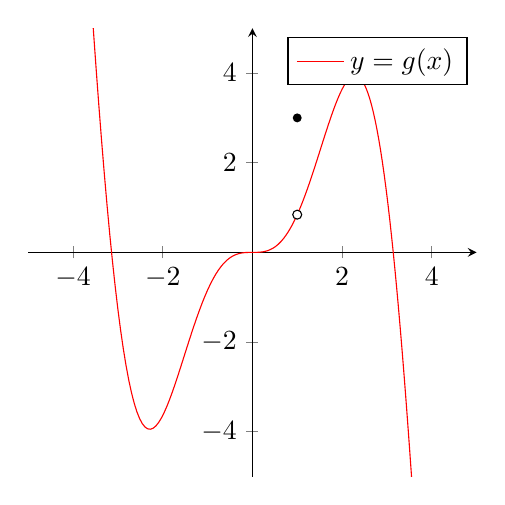
\begin{tikzpicture}
                \begin{axis}[
                    axis lines = center,
                    axis equal image,
                    xmin = -5,
                    xmax = 5,
                    ymin = -5,
                    ymax = 5,
                ]
                %g(x), x<1
                \addplot [
                    domain = -5:1,
                    samples = 100,
                    color = red
                ]
                {sin(deg(x))*x^2};
                \addlegendentry{$y=g(x)$}
                %g(x), x>1
                \addplot[
                    domain = 1:5,
                    samples = 100,
                    color = red
                ]
                {sin(deg(x))*x^2};
                %undefined circle at x = 1
                \path[
                    draw = black,
                    fill = white,
                ]
                (1,0.84147) circle [radius = 0.1];
                %defined circle at x = 1
                \fill[black] (1,3) circle [radius = 0.1];
                \end{axis}
            \end{tikzpicture}
        \end{center}

        \noindent \color{purple} \textbf{Infinite Discontinuities:} \color{black} \\
        Infinite discontinuities always occur at vertical asymptotes. There may be a vertical
        asymptote at either one or both sides of the function. An example of an infinite
        discontinuity is given below, where $y=h(x)$. \\

        \begin{center}
            \begin{tikzpicture}
                \begin{axis}[
                    axis lines = center,
                    axis equal image,
                    xmin = -5,
                    xmax = 5,
                    ymin = -3,
                    ymax = 7,
                ]
                %h(x)
                \addplot [
                    samples = 100,
                    color = red
                ]
                {1/((x-1)^2)};
                \addlegendentry{$y=h(x)$}
                %asymptote
                \draw[
                    dashed
                ]
                (1,-3) -- (1,7);
                \end{axis}
            \end{tikzpicture}
        \end{center}

        \noindent Here is an example of an \color{purple} \textbf{Infinite Oscillation Discontinuity}.
        \color{black} \\

        \begin{center}
            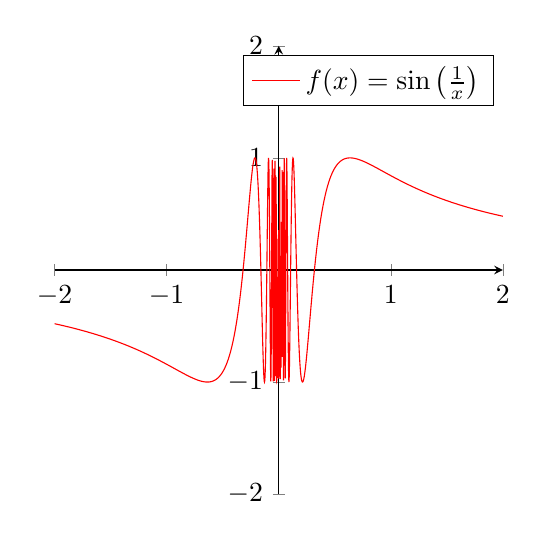
\begin{tikzpicture}
                \begin{axis}[
                    axis lines = center,
                    axis equal image,
                    xmin = -2,
                    xmax = 2,
                    ymin = -2,
                    ymax = 2,
                ]
                %f(x)
                \addplot [
                    samples = 5000,
                    color = red
                ]
                {sin(deg(1/x))};
                \addlegendentry{$f(x)=\sin{\left(\frac{1}{x}\right)}$}
                \end{axis}
            \end{tikzpicture}
        \end{center}

        \noindent \color{purple} \textbf{Essential Discontinuities} \color{black} are discontinuities
        that at which the limit of the function does not exist. Jump and infinite discontinuities
        are essential discontinuities. \\\\

        \noindent Below is a general example about continuity and discontinuity. \\
        \color{blue} \textit{Example: Is} \\

        \begin{equation*}
            f(x)=\begin{cases}
            {
            x^2+2 & x\leq 1 \\
            4 & x > 1
            }
            \end{cases}
        \end{equation*}

        \noindent continuous at $x=1$? \color{black} \\
        Since $\lim_{x\to 1^-}f(x)=3\not=\lim_{x\to 1^+}f(x)=4$.

    \subsection{The Extreme Value Theorem}
        This theorem is best learnt after derivatives. \\
        \color{purple} \textbf{The Extreme Value Theorem} \color{black} \\
        If real numbers $a$ and $b$ satisfy $a<b$ and a function $f$ is continuous on $[a,b]$,
        then $f$ attains a maximum and minimum value on $[a,b]$. \\

        \noindent \color{blue} \textit{Example: Find the maximum and minimum values of the
        function $f(x)=x^3-\frac{9}{2}x^2-12x+20$ on the interval $[-2,6]$}. \color{black} \\
        $f(x)$ is differentiable, hence continuous on the closed and bounded interval. Having
        satisfied the preconditions, we can apply the EVT to this context. Taking the first
        derivative of $f(x)$, we get \\

        \begin{align*}
            f'(x) &= 3x^2 -9x -12 \\
            &= 3(x^2-3x-4)
        \end{align*}

        \noindent Setting $f'(x)=0$ and solving, we find that the critical points are $x=-1,4$
        which by the first derivative test gives the relative extrema $y=26.5,-36$, respectively.
        Computing the endpoints, we have $f(-2)=18$ and $f(6)=2$. Hence, the minimum value of $f$
        on $[-2,6]$ is -36 and the maximum value is 26.5.



    \subsection{The Intermediate Value Theorem}
        \color{purple} \textbf{The Intermediate Value Theorem:} \color{black} \\
        If a function $f$ is continuous on the closed interval $[a,b]$, and $M$ is a number such
        that $f(a)\leq M\leq f(b)$, then there is at least one number $c$ such that $f(c)=M$. \\

        \noindent \color{blue} \textit{Example: Does a $x$ exist for some $x\in[0,2]$ such that
        the function $f(x)=x^2+\cos{(\pi x)}=4$?} \color{black} \\

        \begin{align*}
            f(0) = 0^2 + \cos{0} = 1 \\
            f(2) = 2^2 + \cos{2\pi} = 5
        \end{align*}

        \noindent Since $f(0)=1<4<5=f(2)$ and $f$ is continuous, the IVT implies that $f(x)=4$
        for some $x\in[0,2]$.



    \subsection{The Continuous Functions Theorem}
        \color{purple} \textbf{The Continuous Functions Theorem:} \color{black} \\
        If functions $f$ and $g$ are both continuous at $x=c$, then the following functions are
        also continuous: \\

        \begin{tabular}{cc}
            Constant Multiples: & $k\cdot f(x)$ for any real number $k$ \\
            Sums: & $f(x)+g(x)$ \\
            Differences: & $f(x)-g(x)$ \\
            Products: & $f(x)\cdot g(x)$ \\
            Quotients: & $\frac{f(x)}{g(x)}, g(c)\not=0$
        \end{tabular}



    \subsection{The Composition of Continuous Functions Theorem}
        \color{purple} \textbf{The Composition of Continuous Functions Theorem:} \color{black} \\
        If the function $g$ is continuous at $x=c$ and the function $f$ is continuous at $x=g(c)$,
        then the composite function $(f\circ g)(x)$ is continuous at $x=c$.  % Linear Functions
    \section{Differentiation}

    \subsection{Rates of Change and Derivatives}
        An \textbf{average rate of change} describes the overall
        $\frac{\text{rise}}{\text{run}}$-value over an interval $[a,b]$. Geometrically,
        this can be represented by the slope of a secant line through $f(a)$ and $f(b)$ of a
        function $f(x)$. In the graph below, the average rate of change between $x=0$ and
        $x=2$ is given by \\

        \begin{equation*}
            m_{\text{avg}} = \frac{f(b)-f(a)}{b-a} = \frac{4-0}{2-0} = 2
        \end{equation*}

        \begin{center}
            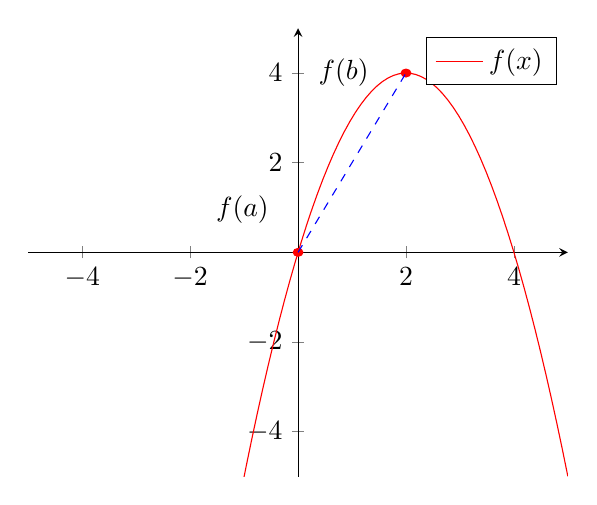
\begin{tikzpicture}
                \begin{axis} [
                    axis lines = center,
                    xmin = -5,
                    xmax = 5,
                    ymin = -5,
                    ymax = 5
                ]
                %f(x)
                \addplot[
                    color = red,
                    samples = 100,
                ]
                {-(x-2)^2+4};
                \addlegendentry{$f(x)$}
                %f(a)
                \fill[red] (0,0) circle [radius = 0.1];
                \node [
                    above left = 10pt of {(0,0)}
                ]
                {$f(a)$};
                %f(b)
                \fill[red] (2,4) circle [radius = 0.1];
                \node[
                    left = 10pt of
                    {(2,4)}
                ]
                {$f(b)$};
                %secant
                \draw [
                    dashed,
                    color = blue
                ]
                (0,0) -- (2,4);
                \end{axis}
            \end{tikzpicture}
        \end{center}

        \noindent A derivative is an \textbf{instantaneous rate of change}, or the slope of the
        tangent to a function at a particular point, $a$. Derivatives are always taken
        \textit{with respect} to a variable. For example, a derivative representing the
        instantaneous rate of change between distance and time is a derivative of distance
        with respect to time, the independent variable. For reference, the derivative of a
        function $f(x)$ at $x=1$ is shown in the graph below. \\

        \begin{center}
            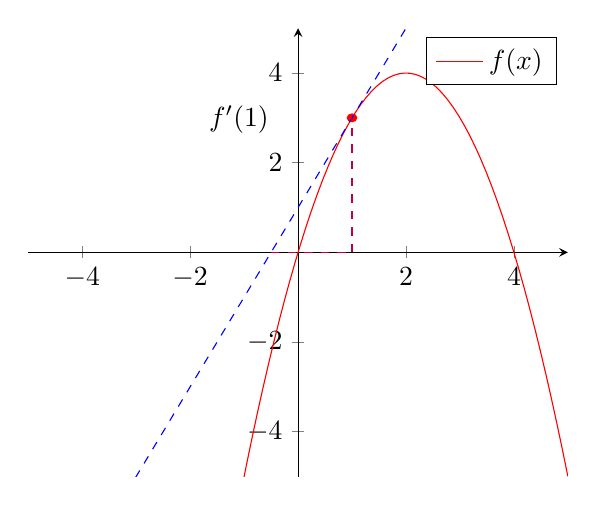
\begin{tikzpicture}
                \begin{axis} [
                    axis lines = center,
                    xmin = -5,
                    xmax = 5,
                    ymin = -5,
                    ymax = 5
                ]
                %f(x)
                \addplot[
                    color = red,
                    samples = 100,
                ]
                {-(x-2)^2+4};
                \addlegendentry{$f(x)$}
                %f(1)
                \fill[red] (1,3) circle [radius = 0.1];
                \node [
                    above left = 10pt of {(0,2)}
                ]
                {$f'(1)$};
                %tangent
                \draw [
                    dashed,
                    color = blue
                ]
                (5,11) -- (-5,-9);
                %rise
                \draw[
                    dashed,
                    color = purple
                ]
                (1,0) -- (1,3);
                %run
                \draw[
                    dashed,
                    color = purple
                ]
                (-0.5,0) -- (1,0);
                \end{axis}
            \end{tikzpicture}
        \end{center}

        \noindent Since the derivative is an instantaneous rate of change, we can define the
        derivative as below. \\
        \color{purple} \textbf{$1^{st}$ Limit Definition of the Derivative} \color{black} \\
        The derivative of $f(x)$ with respect to $x$ is the function $f'(x)$, defined as \\

        \begin{equation*}
            f'(x) = \lim_{x\to a} \frac{f(x)-f(a)}{x-a}
        \end{equation*}

        \noindent Then, if we let $x=a+h$ and change the variable of inspection from $a$ to $x$,
        we can realize the most commonly used definition of the derivative, given below. This
        definition is preferred to the above definition, as finding the derivative only requires
        one value of $x$, rather than 2.  \\
        \color{purple} \textbf{$2^{nd}$ Limit Definition of the Derivative} \color{black} \\
        The derivative of $f(x)$ with respect to $x$ is the function $f'(x)$, defined as \\

        \begin{equation*}
            f'(x) = \lim_{h\to 0} \frac{f(a+h)-f(x)}{h}
        \end{equation*}

        \noindent The expression consisting the right side of the equation above is known as the
        \textbf{difference quotient}. \\

        \noindent A function is $f(x)$ is \textbf{differentiable} at $x=a
        $ if $f'(a)$ exists. Since derivatives are defined by limits, for a derivative to exist,
        its limit must also exist. Hence, \\

        \begin{equation*}
            \text{If $f(x)$ is differentiable at $x=a$ then $f(x)$ is continuous at $x=a$}
        \end{equation*}

        \noindent By this, we can also say that differentiability implies continuity. It is
        important to note that its converse is not always true, as not all continuous functions
        are differentiable. \\


        \noindent A few examples of contexts where a derivative may not exist are at vertical
        tangents, corners, and cusps. Take, for example, the graph below, which does not have a
        derivative at $x=0$ since the respective slopes immediately right and left of $x=0$ are
        different. \\

        \begin{center}
            \begin{tikzpicture}
                \begin{axis}[
                    axis lines = center,
                    axis equal image
                ]
                %f(x)
                \addplot [
                    samples = 50,
                    color = red,
                ]
                {abs(x)};
                \addlegendentry{$f(x)=|x|$}
                \end{axis}
            \end{tikzpicture}
        \end{center}

        \noindent \color{purple} \textbf{Derivative Notations:} \\
        \noindent \textbf{Leibniz's Notation:} \color{black} \\
        The Leibniz notation is popular throughout mathematics, most commonly used when the
        equation $y=f(x)$ is regarded as a functional relationship between dependent and
        independent variables $y$ and $x$. Leibniz's notation makes this relationship explicit
        by representing the derivative as \\

        \begin{equation*}
            \frac{dy}{dx}=\frac{d}{dx}y
        \end{equation*}

        \noindent The Leibniz notation is also called \textbf{differential notation}, where
        $dy$ and $dx$ are \textbf{differentials}. Where the function $y=f(x)$, we can write \\

        \begin{equation*}
            \frac{df}{dx}(x)=\frac{df(x)}{dx}=\frac{d}{dx}f(x)
        \end{equation*}

        \noindent A \textbf{differential equation} is an equation relating one or more functions
        and their derivatives. As long as the precondition ($f(x)$ is satisfied), a function can
        be differentiated indefinite times. For example, in physics, acceleration is the
        derivative of velocity, the derivative of position. The \textbf{order} of a differential
        equation is the highest derivative of said equation. Higher-order derivatives can be
        written in the Leibniz's notation as \\

        \begin{equation*}
            \frac{d^2y}{dx^2}, \frac{dy^3}{dx^3}, \frac{dy^4}{dx^4},\dots,\frac{d^ny}{dx^n}
        \end{equation*}

        \noindent With Leibniz's notation, the value of a derivative at a particular point, $a$,
        can be expressed as \\

        \begin{equation*}
            \frac{dy}{dx}\Bigr|_{x=a}
        \end{equation*}

        \noindent This notation is particularly useful in expressing partial derivatives
        (covered later) and making the chain rule intuitive: \\

        \begin{equation*}
            \frac{dy}{dx} = \frac{dy}{du}\cdot\frac{du}{dx}
        \end{equation*}

        \noindent \color{purple} \textbf{Lagrange's Notation:} \color{black} \\
        In Lagrange's notation, each prime mark denotes a derivative. For higher-order derivatives,
        the order is enclosed by parantheses in front and above the function. \\

        \begin{equation*}
            f'(x), f''(x), f'''(x), f^{(4)}(x),f^{(5)}(x),f^{(6)}(x),f^{(n)}(n)
        \end{equation*}

        \noindent \color{purple} \textbf{Newton's Notation:} \color{black} \\

        This notation is often applied to physics contexts, where time ($t$) is the independent
        variable. The number of dots over the dependent variable represent the order the
        derivative is in. If $y$ is a function of $t$, then the first $n$ derivatives of
        the function are as below. \\

        \begin{equation*}
            \dot{y}, \ddot{y}, \dddot{y}, _{\dot{y}}^4, _{\dot{y}}^5, _{\dot{y}}^n
        \end{equation*}

        \noindent \color{purple} \textbf{Euler's Notation:} \color{black} \\
        This notation is quite inconvenient, as it leaves the variable being differentiated with
        respect to entirely implicit. However, we can modify the notation to explicitly write
        said variable. This notation is defined by \\

        \begin{equation*}
            (Df)(x) = \frac{df(x)}{dx}
        \end{equation*}

        \pagebreak
        \noindent Higher-order Derivatives are expressed by \\

        \begin{equation*}
            D^2f=D^2_xf, D^3f=D^3_xf, D^nf=D^n_xf
        \end{equation*}

        \noindent \color{blue} \textit{Example 1: Find the derivative, $g'(t)$, given the function} \\

        \begin{equation}
            g(t) = \frac{t}{t+1}
        \end{equation} \color{black}

        \begin{align*}
            g'(t) &= \lim_{h\to 0} \frac{g(t+h)-g(t)}{h} \\
            &= \lim_{h\to 0} \frac{1}{h}\left(\frac{t+h}{t+h+1}-\frac{t}{t+1}\right) \\
            &= \lim_{h\to 0}\left(\frac{(t+h)(t+1)-t(t+h+1)}{(t+h+1)(t+1)}\right) \\
            &= \lim_{h\to 0} \frac{1}{h}\left(\frac{t^2+t+th+h-(t^2+th+t)}{(t+h+1)(t+1)}\right) \\
            &= \lim_{h\to 0} \frac{1}{h} \left(\frac{h}{(t+h+1)(t+1)}\right) \\
            &= \frac{1}{(t+1)(t+1)} \\
            g'(t) &= \frac{1}{(t+1)^2}
        \end{align*}

        \noindent \color{blue} \textit{Example 2: Find the derivative, $f'(x)$, of } \\

        \begin{equation*}
            f(x) = 2x^2-16x+35
        \end{equation*} \color{black}

        \begin{align*}
            f'(x) &= \lim_{h\to 0} \frac{2(x+h)^2-16(x+h)+35-(2x^2-16x+35)}{h} \\
            &= \lim_{h\to 0} \frac{4xh+2h^2-16h}{h} \\
            &= \lim_{h\to 0} (4x+2h-16) \\
            f'(x) &= 4x-16
        \end{align*}


    \subsection{Basic Derivative Rules}
        \begin{center}
            \begin{tabular}{|c|c|}
                \hline
                $\frac{d}{dx}a = 0$ & \textbf{Constant} \\
                \hline
                $\frac{d}{dx}au = a\frac{du}{dx}$ & \textbf{Constant Multiple} \\
                \hline
                $\frac{d}{dx}x^n=nx^{n-1}$ & \color{purple} \textbf{The Power Rule} \color{black} \\
                \hline
                $\frac{d}{dx}(u\pm v) = \frac{d}{dx}u \pm \frac{d}{dx}v$ & \textbf{Sum/Difference}\\
                \hline
                $\frac{d}{dx}(uv) = u\frac{dv}{dx}+v\frac{du}{dx}$ & \color{purple}
                \textbf{The Product Rule} \color{black} \\
                \hline
                $\frac{d}{dx}\left(\frac{u}{v}\right)=\frac{v\frac{du}{dx}-u\frac{dv}{dx}}{v^2},
                v\not = 0$ & \color{purple} \textbf{The Quotient Rule} \color{black} \\
                \hline
                $[f^{-1}]'(b)=\frac{1}{f'(a)}$ & \textbf{Inverse Functions} \\
                \hline
                $\frac{d}{dx}[f^{-1}(x)]=\frac{1}{f'(f^{-1}(x))}=\frac{1}{\frac{dy}{dx}}$ &
                \textbf{Alternate Inverse Functions} \\
                \hline
                $\frac{d(1/f)}{dx}=-\frac{1}{f^2}\frac{df}{dx}$ & \textbf{Reciprocal} \\
                \hline
            \end{tabular}
        \end{center}


    \subsection{Derivatives of Exponential and Logarithmic Functions}
        \begin{center}
            \begin{tabular}{|c|c|}
                \hline
                $\frac{d}{dx}e^x=e^x$ & \textbf{Natural Exponent} \\
                \hline
                $\frac{d}{dx}\ln{x}=\frac{1}{x}$ & \textbf{Natural Logarithm} \\
                \hline
                $\frac{d}{dx}a^x=a^x\ln{a}$ & \textbf{Exponent} \\
                \hline
                $\frac{d}{dx}\log_b{x}=\frac{1}{x\ln{b}}$ & \textbf{Logarithm} \\
                \hline
                $\frac{d}{dx}x^x=x^x(1+\ln{x})$ & \\
                \hline
            \end{tabular}
        \end{center}


    \pagebreak
    \subsection{Derivatives of the Trigonometric Functions}
        The derivatives of $\sin{x}$ and $\cos{x}$ help us derive the others through applying
        the quotient and reciprocal differentiation rules. \\

        \begin{center}
            \begin{tabular}{|c|}
                \hline
                $\frac{d}{dx}\sin{x}=\cos{x}$ \\
                \hline
                $\frac{d}{dx}\cos{x}=-\sin{x}$ \\
                \hline
                $\frac{d}{dx}\tan{x}=\sec^2{x}$ \\
                \hline
                $\frac{d}{dx}\csc{x}=-\cot{x}\csc{x}$ \\
                \hline
                $\frac{d}{dx}\sec{x}=\tan{x}\sec{x}$ \\
                \hline
                $\frac{d}{dx}\cot{x}=-\csc^2{x}$ \\
                \hline
            \end{tabular}
        \end{center}

        \noindent The derivatives of the inverse trigonometric functions can be derived through
        applying the inverse differentiation rule. \\

        \begin{center}
            \begin{tabular}{|c|}
                \hline
                $\frac{d}{dx}\arcsin{x} = \frac{1}{\sqrt{1-x^2}}$ \\
                \hline
                $\frac{d}{dx}\arccos{x} = -\frac{1}{\sqrt{1-x^2}}$ \\
                \hline
                $\frac{d}{dx}\arctan{x} = \frac{1}{1+x^2}$ \\
                \hline
                $\frac{d}{dx}\arccsc{x} = -\frac{1}{|x|\sqrt{x^2-1}}$ \\
                \hline
                $\frac{d}{dx}\arcsec{x} = \frac{1}{|x|\sqrt{x^2-1}}$ \\
                \hline
                $\frac{d}{dx}\arccot{x} = -\frac{1}{1+x^2}$ \\
                \hline
            \end{tabular}
        \end{center}


        \noindent \color{purple} \textbf{Derivation of the Inverse Sine Derivative:} \color{black} \\
        \begin{align*}
            \frac{d(\arcsin{x})}{dx} &= \frac{1}{\frac{d(\sin{y})}{dy}} \\
            &= \frac{1}{\cos{y}} \\
        \end{align*}
        \noindent From the Pythagorean Identity, \\
        \begin{align*}
            \cos^2{y} + \sin^2{y} &= 1 \\
            \cos^2{y} &= 1 - \sin^2{y} \\
            \cos{y} &= \sqrt{1-\sin^2{y}}
        \end{align*}
        \noindent Substituting this back into the original equation, we get \\
        \begin{align*}
            \frac{d(\arcsin{x})}{dx} &= \frac{1}{\sqrt{1-\sin^2{y}}}
        \end{align*}
        \noindent By the definition of the inverse sine function, we can express the equation as \\
        \begin{align*}
            \frac{d}{dx}\arcsin{x} &= \frac{1}{\sqrt{1-x^2}}
        \end{align*}

        \noindent \color{purple} \textbf{Derivation of the Inverse Cosine Derivative} \color{black} \\
        The derivatives of the inverse trigonometric functions are the \textit{negatives} of the
        derivatives of their cofunctions. This is because \\

        \begin{align*}
            \arccos{x} &= \frac{\pi}{2} - \arcsin{x} \\
            \frac{d}{dx}\arccos{x} &= -\frac{d}{dx}\arcsin{x} \\
            &= -\frac{1}{\sqrt{1-x^2}}
        \end{align*}

        \noindent \color{purple} \textbf{Derivation of the Inverse Tangent Derivative} \color{black} \\

        \begin{align*}
            \frac{d}{dx}\arctan{x} &= \frac{1}{\frac{d(\tan{y})}{dy}} \\
            &= \frac{1}{\sec^2{y}} \\
            &= \frac{1}{1+\tan^2{y}} \\
            &= \frac{1}{1+x^2}
        \end{align*}

    \pagebreak
    \subsection{The Chain Rule}
        The Chain Rule is incredibly useful for finding the derivative of composite functions.
        If $y=f(u)$ and $u=g(x)$ then \\

        \begin{align*}
            (f(g(x)))' &= f'(g(x)) \cdot g'(x) \\
            &= f'(u) \cdot g'(x) \\
            \frac{dy}{dx} &= \frac{dy}{du} \cdot \frac{du}{dx}
        \end{align*}

        \noindent \color{blue} \textit{Example 1:} \color{black} \\

        \begin{align*}
            f(x) &= \sqrt{5x-8} \\
        \end{align*}

        \noindent We let the inside function be expressed as $u=5x-8$. Then \\

        \begin{align*}
            f'(x) &= \frac{du}{dx}u^{\frac{1}{2}}\cdot\frac{dy}{du}(5x-8) \\
            &= \frac{1}{2\sqrt{u}}\cdot 5 \\
            &= \frac{5}{2\sqrt{5x-8}}
        \end{align*}

        \noindent \color{blue} \textit{Example 2:} \color{black} \\
        \noindent Let $u=\cos{t}$ and $v=t^4$

        \begin{align*}
            g(t) &= \cos^4{t} + \cos{(t^4)} \\
            g'(t) &= \frac{d(u^4)}{du} \cdot \frac{d}{dt}\cos{t}
            +
            \frac{d(t^4)}{dt} \cdot \frac{d(\cos{v})}{dv} \\
            &= 4u^3(-\sin{t}) + 4t^3(-\sin{v}) \\
            &= -4\cos^3{t}\sin{t} - 4t^3\sin{(t^4)}
        \end{align*}

    \subsection{Implicit Differentiation}
        \color{purple} \textbf{Implicit Differentiation} \color{black} is an approach to
        differentiating a function that may not be in the explicit form, $y=f(x)$. It
        considers all other variables as functions of one of its variables, then uses the
        chain rule to find the derivative. \\

        \noindent \color{blue} \textit{Example 1: Given $x^2+x+y^2=15$, what is $\frac{dy}{dx}$
        at the point $(2,3)$?} \color{black} \\

        \begin{align*}
            \frac{dy}{dx}(x^2+x+y^2) &= \frac{dy}{dx}15 \\
            2x + 1 + 2y\left(\frac{dy}{dx}\right) &= 0 \\
            \frac{dy}{dx} &= -\frac{2x+1}{2y} \\
            \frac{dy}{dx}\Bigr|_{(2,3)} &= -\frac{2(2)+1}{2(3)} \\
            &= -\frac{5}{6}
        \end{align*}

        \noindent \color{blue} \textit{Example 2: Find the derivative of
        $\ln{y}+e^y=\sin{y^2}-3\cos{x}$} \color{black} \\

        \begin{align*}
            \frac{dy}{dx}\ln{y} + \frac{dy}{dx}e^y &= \frac{d}{dx}\sin{y^2}-\frac{d}{dx}3\cos{x} \\
            \frac{d}{dy}\ln{y}\cdot\frac{dy}{dx}+\frac{d}{dy}e^y\cdot\frac{dy}{dx}
            &= \frac{d}{dy}\sin{y^2}\cdot\frac{dy}{dx}+3\sin{x} \\
            \frac{dy}{dx}\left(\frac{1}{y}+e^y-2y\cos{y^2}\right) &= 3\sin{x} \\
            \frac{dy}{dx} &= \frac{3\sin{x}}{\frac{1}{y}+e^y-2y\cos{y^2}}
        \end{align*}

        \noindent \color{blue} \textit{Example 3: Find $\frac{dy}{dx}$ if $y^2 &= x^2 + \sin{(xy)}$}
        \color{black} \\

        \begin{align*}
            \frac{d}{dx}(y^2) &= \frac{d}{dx}(x^2) + \frac{d}{dx}(\sin{(xy)} \\
            2y\frac{d}{dx} &= 2x + (\cos{(xy)})\left(y+x\frac{d}{dx}\right) \\
            (2y-x\cos{(xy)})\frac{d}{dx} &= 2x + y\cos{(xy)} \\
            \frac{dy}{dx} &= \frac{2x+y\cos{(xy)}}{2y-x\cos{(xy)}}
        \end{align*}


    \subsection{Logarithmic Differentiation}
        This method of finding derivatives uses the basic properties of logarithms outside
        of calculus to simply a function prior to differentiating it. \\

        \noindent \color{blue} \textit{Example 1:} \color{black} \\

        \begin{align*}
            y &= \frac{x^5}{(1-10x)\sqrt{x^2+2}} \\
            \ln{y} &= \ln{\left(\frac{x^5}{(1-10x)\sqrt{x^2+2}}\right)} \\
            &= \ln{(x^5)} - \ln{\left((1-10x)\sqrt{x^2+2}\right)} \\
            &= \ln{(x^5)} - \ln{(1-10x)} - \ln{(\sqrt{x^2+2})}
        \end{align*}

        \noindent By Implicit Differentiation, \\

        \begin{align*}
            \fra{y'}{y} &= \frac{5x^4}{x^5}- \frac{-10}{1-10x} - \frac{\frac{1}{2}(x^2+2)^{-\frac{1}{2}}(2x)}{(x^2+2)^{\frac{1}{2}}} \\
            &= \frac{5}{x} + \frac{10}{1-10x} - \frac{x}{x^2+2} \\
            \frac{dy}{dx} &= \frac{x^5}{(1-10x)\sqrt{x^2+2}}\left(\frac{5}{x}+\frac{10}{1-10x}-\frac{x}{x^2+2}\right)
        \end{align*}

        \noindent \color{blue} \textit{Example 2:} \color{black} \\

        \begin{align*}
            y &= \frac{x+3}{(x+4)^3} \\
            \ln{y} &= \ln{\left(\frac{x+3}{(x+4)^3}\right)} \\
            &= \ln{(x+3)} - \ln{(x+4)^3} \\
            &= \ln{(x+3)}  - 3\ln{(x+4)} \\
            \frac{1}{y}\cdot\frac{dy}{dx} &= \frac{1}{x+3}-3\cdot\frac{1}{x+4} \\
            &= \frac{1}{x+3}-\frac{3}{x+4} \\
            \frac{dy}{dx} &= y\left(\frac{1}{x+3}-\frac{3}{x+4}\right)
        \end{align*}


    \subsection{Derivatives of Parametric Functions}
        If $x=f(t)$ and $y=g(t)$ are differentiable functions of parameter $t$, then \\

        \begin{equation*}
            \frac{dy}{dx} = \frac{\frac{dy}{dt}}{\frac{dx}{dt}}
        \end{equation*}

        \noindent and

        \begin{equation*}
            \frac{d^2y}{dx^2} = \frac{d}{dx}\left(\frac{dy}{dx}\right)
            = \frac{\frac{d}{dt}\left(\frac{dy}{dx}\right)}{\frac{dx}{dt}}
        \end{equation*}

        \noindent \color{blue} \textit{Example: If $x=2\sin{\theta}$ and $y=\cos{2\theta}$,
        find $\frac{d^2y}{dx^2}$} \color{black} \\

        \begin{align*}
            \frac{dy}{dx} &= \frac{\frac{dy}{d\theta}}{\frac{dx}{d\theta}} \\
            &= \frac{-2\sin{2\theta}}{2\cos{\theta}} \\
            &= -\frac{2\sin\theta\cos\theta}{\cos\theta} \\
            &= -2\sin\theta
        \end{align*}

        \begin{align*}
            \frac{d^2y}{dx^2} &= \frac{\frac{d}{d\theta}\left(\frac{dy}{dx}\right)}{\frac{dx}{d\theta}} \\
            &= \frac{-2\cos\theta}{2\cos\theta} \\
            &= -1
        \end{align*}



    \subsection{Derivatives of Polar Functions}
        We know that $x=r\cos\theta$ and $y=r\sin\theta$. Then, by using the parametric derivative
        formula, we can determine the rule for differentiating polar functions. \\

        \begin{align*}
            \frac{dy}{dx} &= \frac{\frac{dy}{d\theta}}{\frac{dx}{d\theta}} \\
            &= \frac{f'(\theta)\sin\theta+f(\theta)\cos\theta}{f'(\theta)\cos\theta-f(\theta)\sin\theta} \\
            &= \frac{r'\sin\theta+r\cos\theta}{r'\cos\theta-r\sin\theta}
        \end{align*}

        \noindent \color{blue} \textit{Example: Find the slope of the cardioid
        $r=2(1+\cos\theta)$ at $\theta=\frac{\pi}{6}$} \color{black} \\

        \begin{align*}
            r=2(1+\cos\theta) \\
            r' = -2\sin\theta
        \end{align*}

        \noindent Then \\

        \begin{align*}
            \frac{dy}{dx} &= \frac{\frac{dy}{d\theta}}{\frac{dx}{d\theta}} \\
            &= \frac{(-2\sin\theta)\sin\theta+2(1+\cos\theta)(\cos\theta)}{(-2\sin\theta)\cos\theta-2(1+\cos\theta)(\sin\theta)} \\
            \frac{dy}{dx}\Bigr|_{\frac{\pi}{6}} &= -1
        \end{align*}



    \subsection{Derivatives of Vector-Valued Functions}
        If a point moves along a curve defined parametrically by $P(t)=\langle x(t), y(t)\rangle$,
        where $t$ represents time, then the vector from the origin to $P$ is called the
        \textbf{position vector}. Then the derivative of the position vector is called the
        \textbf{velocity vector}, and its derivative is called the \textbf{acceleration vector}.  \\

        \noindent \color{purple} \textbf{The Velocity Vector:} \color{black} \\

        \begin{equation*}
            \overrightarrow{v}(t) = \left\langle\frac{dx}{dt},\frac{dy}{dt}\right\rangle
        \end{equation*}

        \noindent The slope of $\overrightarrow{v}$ is given by \\

        \begin{equation*}
            \frac{dy}{dx} = \frac{\frac{dy}{dt}}{\frac{dx}{dt}}
        \end{equation*}

        \noindent \color{purple} \textbf{The Magnitude of a Velocity Vector:} \color{black} \\

        \begin{equation*}
            |v| = \sqrt{\left(\frac{dx}{dt}\right)^2+\left(\frac{dy}{dt}\right)^2} = \sqrt{v^2_x+v^2_y}
        \end{equation*}

        \noindent \color{purple} \textbf{The Acceleration Vector:} \color{black} \\

        \begin{equation*}
            \overrightarrow{a}(t) = \left\langle\frac{d^2x}{dt^2},\frac{d^2y}{dt^2}\right\rangle
        \end{equation*}

        \noindent \color{purple} \textbf{The Magnitude of an Acceleration Vector:} \color{black} \\

        \begin{equation*}
            |a| = \sqrt{\left(\frac{d^2x}{dt^2}\right)^2+\left(\frac{d^2y}{dt^2}\right)^2} = \sqrt{a^2_x+a^2_y}
        \end{equation*}



    \subsection{Rolle's Theorem}
        \color{purple} \textbf{Rolle's Theorem:} \color{black} \\
        \noindent Suppose $f(x)$ is a function that is both continuous on the closed interval
        $[a,b]$ and differentiable on the open interval $(a,b)$, and that $f(a)=f(b)$.
        Then there is a number $c$ such that $a<c<b$ and $f'(c)=0$. Or rather, $f(x)$ has a
        critical point in $(a,b)$. \\



    \subsection{The Mean Value Theorem}
        \color{purple} \textbf{The Mean Value Theorem:} \color{black} \\
        \noindent Suppose $f(x)$ is a function that is both continuous on the closed interval
        $[a,b]$ and differentiable on the open interval $(a,b)$. Then there is a number
        $c$ such that $a<c<b$ and \\

        \begin{equation*}
            f'(c) = \frac{f(b)-f(a)}{b-a}
        \end{equation*}

        \noindent Or, \\

        \begin{equation*}
            f(b) - f(a) = f'(c) (b-a)
        \end{equation*}

        \noindent \color{blue} \textit{Example 1: Determine all the numbers $c$ satisfying
        $f(x)=x^3+2x^2-x$ on $[-1,2]$} \color{black} \\

        \begin{align*}
            f'(x) &= 3x^2+4x-1 \\
            f'(c) &= \frac{f(2)-f(-1)}{2-(-1)} \\
            3c^2+4c-1 &= \frac{14-2}{3} \\
            3c^2+4c-1 &= 4 \\
            3c^2+4c-5 &= 0 \\
            c &= \frac{-4\pm\sqrt{16-4(3)(-5)}}{6} \\
            c &= 0.7863, -2.1196 \\
            c &= 0.7863
        \end{align*}

        \noindent Notice we were able to remove the other $c$, as it is outside of the desired interval.

        \noindent \color{blue} \textit{Example 2: Suppose we know that $f(x)$ is continuous and
        differentiable on $[6,15]$ and that $f(6)=-2$ and $f'(x)\leq10$. Find the
        largest possible value for $f(15)$.} \color{black} \\

        \noindent The MVT tells us that \\

        \begin{equation*}
            f(15) - f(6) = f'(c)(15-6)
        \end{equation*}

        \noindent Plugging in known quantities and simplifying, we get \\

        \begin{equation*}
            f(15) = -2 + 9f'(c)
        \end{equation*}

        \noindent Since we are given $f'(x)\leq 10$, we know that $f'(c)\leq 10$. This gives us \\

        \begin{align*}
            f(15) &= -2 + 9f'(c) \\
            &\leq -2 + (9)10 \\
            &\leq 88
        \end{align*}

        \noindent Hence, the largest possible value of $f(15)=88$.  % Quadratic Functions
    \section{Applications of Differentiation}

    \subsection{Critical Points}
        $x=c$ is a \textbf{critical point} of the function $f'(x)$ if $f(c)$ exists and \\

        \begin{center}
            \begin{tabular}{ccc}
                $f'(c) = 0$ & OR & $f'(c)$ doesn't exist
            \end{tabular}
        \end{center}

        \noindent \color{blue} \textit{Example: Determine all the critical points for the function} \\

        \begin{equation*}
            f(x) = 6x - 4\cos{(3x)}
        \end{equation*} \color{black} \\

        \begin{align*}
            f'(x) = 0 &= 6 + 12\sin{(3x)} \\
            \sin{(3x)} &= -\frac{1}{2} \\
            x &= 1.2217+\frac{2\pi n}{3}, n=0,\pm 1,\pm 2,\dots \\
            \text{and} \\
            x &= 1.9199+\frac{2\pi n}{3}, n=0,\pm 1,\pm 2,\dots
        \end{align*}


    \subsection{Tangents to Curves}
        Recall the point-slope form of a linear function from Algebra. We can replace the slope,
        $m$, with $f'(x_1)$ to get an equation of the tangent to the curve $y=f(x)$ at point
        $P(x_1,y_1)$. \\

        \noindent \color{purple} \textbf{Equation for Tangent to a Curve} \color{black} \\

        \begin{equation*}
            y - y_1 = f'(x_1)(x-x_1)
        \end{equation*}

        \noindent \color{blue} \textit{Example: Find an equation of the tangent to
        $f(t)=(\cos{t}, 2\sin^2{t})$ at the point where $t=\frac{\pi}{3}$} \color{black} \\

        \begin{align*}
            \frac{dy}{dx} &= \frac{\frac{dy}{dt}}{\frac{dx}{dt}} \\
            &= \frac{4\sin{t}{\cos{t}}}{-\sin{t}} \\
            &= -4\cos{t}
        \end{align*}

        \noindent At $t=\frac{\pi}{3}$, $x=\frac{1}{2}$,
        $y=2\left(\frac{\sqrt{3}}{2}\right)^2=\frac{3}{2}$, and $\frac{dy}{dx}=-2$.
        Hence, an equation of the tangent is \\

        \begin{align*}
            y - \frac{3}{2} &= -2\left(x-\frac{1}{2}\right) \\
            4x + 2y &= 5
        \end{align*}


    \subsection{Increasing and Decreasing Functions}
        A function $f(x)$ is \textbf{increasing} on an interval for which $a<b$, $f(b)\geq f(a)$.
        A function $f(x)$ is \textbf{decreasing} over an interval for which $a<b$, $f(b)\leq f(a)$.
        Hence, the following identities hold true. \\

        \begin{center}
            \begin{tabular}{|c|c|}
                \hline
                $f'(x)>0$ & Increasing \\
                \hline
                $f'(x)<0$ & Decreasing \\
                \hline
            \end{tabular}
        \end{center}

        \noindent \color{blue} \textit{Example: For what values of $x$ is $f(x)=x^4-4x^3$
        increasing and decreasing, respectively?} \color{black} \\

        \begin{align*}
            f'(x) &= 4x^3 -12x^2 \\
            &= 4x^2(x-3)
        \end{align*}

        \noindent With critical values at $x=0,3$, we analyze the signs of $f'$ in the three
        intervals as below. \\

        \begin{center}
            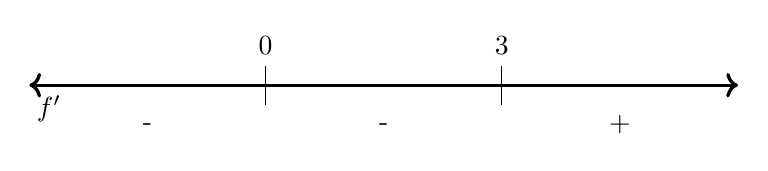
\begin{tikzpicture}
                \draw[<->, very thick] (-4.5,0) -- (4.5,0); %number line
                \draw (-1.5,0.25) -- (-1.5,-0.25); %Vertical tick marks
                \draw (1.5,0.25) -- (1.5,-0.25);
                \node () at (-4.25,-0.3) {$f'$}; %Labels
                \node () at (-1.5,0.5) {0};
                \node () at (1.5,0.5) {3};
                \node () at (-3,-0.5) {-}; %Sign markings
                \node () at (0,-0.5) {-};
                \node () at (3,-0.5) {+};
            \end{tikzpicture}
        \end{center}

        \nonindent Since the derivative changes sign only at $x=3$,\\

        \begin{center}
            \begin{tabular}{cc}
                if $x<3$ & $f'(x)\leq 0$ and $f$ is decreasing \\
                If $x>3$ & $f'(x)> 0$ and $f$ is increasing
            \end{tabular}
        \end{center}


    \subsection{Extrema, Concavity, and Inflection Points}
        The curve of $y=f(x)$ has a \textbf{local/relative maximum} at a point where $x=c$ if
        $f(c)\geq f(x)$ for all $x$ in the immediate neighborhood of $c$. If a curve has a
        relative maximum at $x=c$, then the curve changes from increasing to decreasing as $x$
        increases through $c$. \\

        \noindent The curve of $y=f(x)$ has a \textbf{local/relative minimum} at a point where
        $x=c$ if $f(c)\leq f(x)$ for all $x$ in the immediate neighborhood of $c$.
        If a curve has a relative minimum at $x=c$, then the curve changes from decreasing to
        increasing as $x$ increases through $c$. \\

        \noindent If a function is differentiable on $[a,b]$ and has a relative extremum at $
        x=c, a<c<b$, then $f'(c)=0$. \\

        \noindent The \textbf{global/absolute maximum} of a function on $[a,b]$ occurs at $x=c$
        if $f(c)\geq f(x)$ for all $x$ on $[a,b]$. The \textbf{global/absolute minimum} of a
        function on $[a,b]$ occurs at $x=c$ if $f(c)\leq f(x)$ for all $x$ on $[a,b]$. \\

        \noindent A curve is \textbf{concave upward} on an interval $(a,b)$ if the curve lies
        above the tangent lines at each point in the interval $(a,b)$. A curve is
        \textbf{concave downward} on an interval $(a,b)$ if the curve lies below the tangent
        lines at each point in the interval $(a,b)$. \\

        % @TODO: Last tikzpicture won't load need to fix
        \begin{center}
            \begin{tabular}{|c|c|}
                \hline
                $f"(x) > 0$ & Concave Up \\
                \hline
                $f"(x) < 0$ & Concave Down \\
                \hline
            \end{tabular}

            \begin{tabular}{cc}
                \begin{tikzpicture} [scale = 0.75]
                    \begin{axis}[
                        axis lines = center,
                        xmin = -7,
                        xmax = 15,
                        ymin = 0,
                        ymax = 20
                    ]
                    \addplot[
                        color = red,
                        samples = 100,
                        domain = -7:15
                    ]
                    {((x-4)^2)/(4)+2};
                    \addplot[
                        dashed,
                        color = blue,
                        domain = -1.8:1.8,
                        samples = 2
                    ]
                    {-2*x+6};
                    \addplot[
                        dashed,
                        color = blue,
                        domain = 2.2:5.8,
                        samples = 2
                    ]
                    {2};
                    \addplot[
                        dashed,
                        color = blue,
                        domain = 6.2:9.8,
                        samples = 2
                    ]
                    {2*x-10};
                    \end{axis}
                \end{tikzpicture}
                &
                \begin{tikzpicture} [scale=0.75]
                    \begin{axis}[
                        axis lines = center,
                        xmin = -7,
                        xmax = 15,
                        ymin = 0,
                        ymax = 20
                    ]
                    \addplot[
                        color = red,
                        samples = 100,
                        domain = -7:15
                    ]
                    {((x-4)^2)/(-4)+18};
                    \addplot[
                        dashed,
                        color = blue,
                        domain = -3.8:-0.2,
                        samples = 2
                    ]
                    {3*x+15};
                    \addplot[
                        dashed,
                        color = blue,
                        domain = 2.2:5.8,
                        samples = 2
                    ]
                    {18};
                    \addplot[
                        dashed,
                        color = blue,
                        domain = 8.2:11.8,
                        samples = 2
                    ]
                    {-3*x+39};
                    \end{axis}
                \end{tikzpicture}
            \end{tabular}
        \end{center}



    \subsection{Related Rates}
        Related rates are an application of implicit differentiation that allow us to solve for
        rates of change and other quantities in an applied real-world system, typically growing
        with respect to time. \\

        \noindent \color{blue} \colorit{Example 1: Air is being pumped into a spherical balloon at
        a rate of 5 $\text{cm}^3$/min. Determine the rate at which the radius of the balloon is
        increasing when the diameter of the balloon is 20 cm.} \color{black} \\

        \noindent We are given $\frac{dV}{dt}=5$ and we want to find $\frac{dr}{dt}_{r=10}$. \\
        \noindent Assuming the balloon is perfectly spherical, its volume is given by
        $V=\frac{4}{3}\pi r^3$. Then

        \begin{align*}
            \frac{dV}{dt}        &= 4\pi r^2 \frac{dr}{dt} \\
            5                    &= 4\pi (10)^2 \frac{dr}{dt} \\
            \frac{dr}{dt}_{r=10} &= \frac{1}{80\pi} \text{cm/min}
        \end{align*}

        \noindent \color{blue} \textit{Example 2: A 15 foot ladder is resting against the wall.
        The bottom is initially 10 feet away from the wall and is being pushed towards the wall at
        the rate of $\frac{1}{4}$ ft/sec. How fast is the top of the ladder moving 12 seconds
        after we start pushing?} \color{black} \\

        \noindent Let us first sketch the situation: \\

        \begin{figure}[hbt!]
            \centering
            \includegraphics[scale=0.6]{Resources/Unit3DiffferentiationApps/Related_Rates_1}
        \end{figure}

        \noindent Let the vertical distance between the ground and the ladder be represented by $y$,
        the horizontal distance between the wall and the end of the ladder be represented by $x$,
        and let the length of the ladder be represented by $c=15$. Then from the Pythagorean Theorem,

        \begin{align*}
            x^2 + y^2       &= c^2 = 15 \\
            2xx' + 2yy'     &= 0 \\
            yy'             &= -xx' \\
            \frac{dy}{dt}   &= \frac{-x\cdot\frac{dx}{dt}}{y} \\
            \frac{dy}{dt}   &= \frac{-7(-\frac{1}{4})}{\sqrt{176}} \\
            \frac{dy}{dt}   &= \frac{7}{4\sqrt{1176}} \approx 0.1319 \text{ft/sec}
        \end{align*}

        Notice that we were able to obtain exact values for $x$ and $y$ because
        $x=10+tx'=10-\frac{1}{4}(12) = 7$ and

        \begin{align*}
            x^2+y^2     &=c^2 \\
            49 + y^2    &= 225 \\
            y           &= \sqrt{176}
        \end{align*}

        \noindent \color{blue} \textit{Example 3: Suppose that we have two resistors connected in
        parallel with resistances $R_1$ and $R_2$ measured in $\Omega$. The total resistance $R$
        is then given by}

        \begin{equation*}
            \frac{1}{R} = \frac{1}{R_1} + \frac{1}{R_2}
        \end{equation*}

        \noindent Suppose that $R_1$ is increasing at a rate of 0.4 $\Omega$/min and $R_2$ is
        decreasing at a rate of 0.7 $\Omega$/min. At what rate is $R$ changing when $R_1=80\Omega$
        and $R_2=105\Omega$? \color{black} \\

        \noindent When $R_1=80\Omega$ and $R_2=105\Omega$,

        \begin{align*}
            \frac{1}{R}     &= \frac{1}{80} + \frac{1}{105} \\
            \frac{1}{R}     &= \frac{37}{1680} \\
            R               &= \frac{1680}{37}
        \end{align*}

        \noindent Then

        \begin{align*}
            \frac{1}{R}     &= \frac{1}{R_1} + \frac{1}{R_2} \\
            -\frac{R'}{R^2} &= -\frac{R'_1}{(R_1)^2} - \frac{R'_2}{(R_2)^2} \\
            \frac{dR}{dt}   &= R^2\left(\frac{R'_1}{(R_1)^2}+\frac{R'_2}{(R_2)^2}\right) \\
            \frac{dR}{dt}   &= \left(\frac{1680}{37}\right)\left(\frac{0.4}{80^2}-\frac{0.7}{105^2}\right) \\
            \frac{dR}{dt}   &\approx -0.002045 \Omega\text{/min}
        \end{align*}


    \subsection{Tangent-Line Approximations}
        Given a function $f(x)$ that is differentiable at $x=a$, we know that the slope of the
        tangent line to $f(x)$ at $(a,f(a))$ is $f'(a)$. Thus, the tangent line $L(x)$ through
        $(a,f(a))$ with slope $f'(a)$ has an equation in point-slope form given by

        \begin{equation*}
            L(x) = f(a) + f'(a)(x-a)
        \end{equation*}

        \noindent Below is a graph of the function $y=f(x)$ and its linearization $y=L(x)$.

        \begin{figure}[hbt!]
            \centering
            \includegraphics[scale=0.6]{Resources/Unit3DiffferentiationApps/Linearization}
        \end{figure}

        \pagebreak
        \noindent \color{blue} \textit{Example 1: Determine the linear approximation for
        $f(x)=\sqrt[3]{x}$ at $x=8$. Use the linear approximation to approximate the value of
        $\sqrt[3]{8.05}$} and $\sqrt[3]{25}$. \color{black}

        \begin{align*}
            L(x)        &= f(8) + f'(8)(x-8) \\
            &= 2 + \frac{1}{3}8^{-\frac{2}{3}}(x-8) \\
            &= \frac{1}{12}x + \frac{4}{3} \\
            L(8.05)     &\approx 2.0041667 \\
            L(25)       &\approx 3.4166667
        \end{align*}



    \subsection{The Newton-Raphson Method}
        The \textbf{Newton-Raphson Method} is a way to quickly find an \textit{approximation}
        iteratively for the root of a real-valued function $f(x)=0$. It is founded on the concept
        that a continuous and differentiable function can be approximated by a tangent line to it. \\

        \noindent Suppose you want to find the root of a continuous, differentiable function $f(x)$ and you
        know that the target root is near the point $x_0$. Then with Newton's Method, an approximation
        for the root $x_1$ is given by

        \begin{equation*}
            x_1 = x_0 - \frac{f(x_0)}{f'(x_0)}
        \end{equation*}

        \noindent This method can be repeated as many times as necessary to get the desired accuracy.
        Then the generalization of Newton's Method is given by \\

        \begin{equation*}
            x_{n+1}     = x_n - \frac{f(x_n)}{f'(x_n)}
        \end{equation*}

        \noindent Below is a visual demonstration of Newton's Method.

        \begin{figure}
            \centering
            \includegraphics{Resources/Unit3DifferentiationApps/NewtonsMethod}
        \end{figure}

        \noindent \color{blue} \textit{Example: Find the root of the equation $x^2-4x-7=0$ near
        $x=5$}. \color{black} \\

        \noindent We are given $x_0=5$. Let $f(x)=x^2-4x-7$ and $f'(x)=2x-4$. Then,

        \begin{align*}
            x_1 &= 5 - \frac{5^2-4\cdot5-7}{2\cdot5-4} = 5-\left(\frac{-2}{6}\right)=\frac{16}{3}
            \approx 5.33333 \\
            x_2 &= \frac{16}{3} - \frac{\left(\frac{16}{3}\right)^2-4\left(\frac{16}{3}\right)-7}
            {2\left(\frac{16}{3}\right)-4} = \frac{16}{3}-\frac{\frac{1}{9}}{\frac{20}{3}}
            = \frac{16}{3} - \frac{1}{60} = \frac{319}{60} \approx 5.31667 \\
            x_3 &= \frac{319}{60} - \frac{\left(\frac{319}{60}\right)^2-4\left(\frac{319}{60}\right)-7}
            {2\left(\frac{319}{60}\right)-4} = \frac{319}{60} -
            \frac{\frac{1}{3600}}{\frac{398}{60}} \approx 5.31662
        \end{align*}


    \subsection{Optimization}
        \textbf{Optimization} uses a function's derivatives to find the maximum or
        minimum value of that function. \\

        \noindent \color{blue} \textit{Example 1: We need to enclose a rectangular field with a
        fence. We have 500 feet of fencing material and a building is on one side of the field
        and so won't need any fencing. Determine the dimensions of the field that will enclose the
        largest area.} \color{black} \\

        \noindent Let us first visualize the situation:

        \begin{figure}
            \centering
            \includegraphics[scale=0.4]{Resources/Unit3DifferentiationApps_optimization}
        \end{figure}

        \noindent We want to maximize the area of the field and we only have 500 ft of fencing
        material. So, we represent this system by the following equations:

        \begin{align*}
            \text{Maximize: } A     &= xy \\
            \text{Constraint: } 500 &= x + 2y
        \end{align*}

        \noindent Solving the constraint equation for $x$, we get $x=500-2y$. We can substitute this
        into the area function, giving us \\

        \begin{align*}
            A(y)  &= (500-2y)y \\
            &= 500y-2y^2 \\
            A'(y) &= 500-4y \\
            0     &= 500 - 4y \\
            y     &= 125 \\
            x     &= 500-2(125) = 250
        \end{align*}

        \noindent Thus, the dimensions of the field that wil give the largest area are 250 x 125. \\

        \noindent \color{blue} \textit{Example 2: A manufacturer needs to make a cylinderical can
        that will hold 1.5 litres of liquid. Determine the dimensions of the can that will
        minimize the amount of material used in its constraint.} \color{black} \\

        \noindent We will eventually need the radius and height of the can in terms of a linear
        measurement unit, instead of litres. Thus, the volume, 1.5 litres, becomes 1500 $\text{cm}^3$.

        \begin{align*}
            \text{Minimize:} A      &= 2\pi rh+2\pi r^2 \\
            \text{Constraint:} 1500 &= \pi r^2 h \\
            h                       &= \frac{1500}{\pi r^2} \\
            \implies A(r)           &= 2\pi r\left(\frac{1500}{\pi r^2}\right) + 2\pi r^2 \\
            A(r)                    &= 2\pi r^2 + \frac{3000}{r} \\
            A'(r)                   &= 4\pi r - \frac{3000}{r^2} \\
            A'(r)                   &= \frac{4\pi r^3 - 3000}{r^2} \\
            0                       &= \frac{4\pi r^3 - 3000}{r^2} \\
            r                       &= \sqrt[3]{\frac{750}{\pi}} \\
            r                       &= 6.2035 \\
            h                       &= \frac{1500}{\pi(6.2035)^2} \\
            h                       &= 12.4070
        \end{align*}

        \noindent Thus, the dimensions of the can that will minimize the material required to
        construct the box are a radius of 6.2035 cm and a height of 12.4070 cm.  % Polynomials
    \section{Integration}

    \subsection{Riemann Sums and Definite Integrals}
        \textbf{Riemann Sums} are approximations of a region's area, obtained by summing the
        areas of numerous simplified slices of said region. The area approximation gets better
        if more slices are used to simplify the area. As you can see from the figures below,
        the figure with more and smaller rectangles takes up more of the area we are trying to
        approximate.

        \begin{figure} [hbt!]
            \centering
            \begin{subfigure}[b]{.45\textwidth}
                \includegraphics[scale=0.8]{Resources/Unit4Integration/Riemann1}
            \end{subfigure}
            \begin{subfigure}[b]{.45\textwidth}
                \includegraphics[scale=0.8]{Resources/Unit4Integration/Riemann2}
            \end{subfigure}
        \end{figure}

        \noindent \textbf{Left Riemann Sums} have rectangles that touch the curve with their
        top-left corners, while \textbf{Right Riemann Sums} have rectangles that touch the curve
        with their top-right corners. \textbf{Midpoint Riemann Sums} have rectangles that touch
        the curve with the middle of their top edges. If the graph is increasing on the interval,
        then the left sum is an underestimate and the right sum is an overestimate. If the graph
        is decreasing on the interval, then the left sum is an overestimate and the left sum is
        an underestimate. Conventionally, we use $i=0$ for left and midpoint sums and $i=1$ for
        right sums. \\

        \noindent Subdivisions of Riemann Sums can be \textbf{uniform}, meaning they are of
        equal width, or \textbf{nonuniform}, meaning they are not of equal length. \\

        \noindent \textbf{Trapezoidal Sums} have subdivisions which touch the curve with both of
        its top vertices. The figures below display left, right, midpoint, and trapezoidal sums.

        \begin{figure}[hbt!]
            \centering
            \begin{subfigure}[b]{.45\textwidth}
                \includegraphics[scale=0.8]{Resources/Unit4Integration/Riemann_Left}
            \end{subfigure}
            \begin{subfigure}[b]{.45\textwidth}
                \includegraphics[scale=0.8]{Resources/Unit4Integration/Riemann_Right}
            \end{subfigure}
        \end{figure}

        \begin{figure}[hbt!]
            \centering
            \begin{subfigure}[b]{.45\textwidth}
                \includegraphics[scale=0.8]{Resources/Unit4Integration/Riemann_Mid}
            \end{subfigure}
            \begin{subfigure}[b]{.45\textwidth}
                \includegraphics[scale=0.8]{Resources/Unit4Integration/Riemann_Trapezoid}
            \end{subfigure}
        \end{figure}

        \noindent If $f(x)$ is defined on the closed interval $[a,b]$ and $c_k$ is any point in
        $[x_{k-1}, x_k]$, then a Riemann Sum is defined as

        \begin{equation*}
            \sum_{i=1}^n f(x_i)\Delta x
        \end{equation*}

        \noindent The Riemman Sum of a function is related to the \textbf{definite integral} as
        follows:

        \begin{equation*}
            \lim_{n\rightarrow\infty}\sum^n_{i=1}f(x_i)\Delta x_i = \int^b_a f(x)dx
        \end{equation*}

        \noindent \color{blue} \textit{Example 1: Approximate the area between $f(x)=|x+3|$ and
        the $x$-axis on the interval $[-5,5]$ using a left Riemann sum with 10 equal subdivisions.}
        \color{black} \\

        \noindent The width of each rectangle, $\Delta x$, is given by

        \begin{equation*}
            \Delta x = \frac{5-(-5)}{10} = 1
        \end{equation*}

        \noindent Since we are using left sums, let $i=0$. Since we have 10 equal subdivisions, the other
        indice of our summation will be 9 such that our area is given by $\sum^9_{i=0}$. We now
        want to find $f(x_i)$. Each time $i$ increases by 1, the value of $x_i$ also increases
        by 1. Its initial value is the left endpoint of the interval, which is -5.

        \begin{equation*}
            x_i = -5 + 1i = -5 + i
        \end{equation*}

        \noindent To confirm that $x_i$ gives us the correct first left endpoint, we substitute 0 for $i$:

        \begin{equation*}
            x_0=-5+0=-5
        \end{equation*}

        \noindent Thus,

        \begin{align*}
            f(x)    &= |x+3| \\
            f(x_i)  &= |(-5+i) +3| \\
            A       &= \sum_{i=0}^9 |(-5+i) + 3| \cdot 1 \\
            A       &= \sum_{i=0}^9 |i-2|
        \end{align*}

        \noindent \color{blue} \textit{Example 2: Approximate the area between $f(x)=\cos{(x)}$
        and the $x$-axis on the interval $\left[-\frac{3}{10}\pi, \frac{1}{2}\pi\right]$ using
        a right Riemann sum with 8 equal subdivisions.} \color{black}

        \begin{align*}
            \Delta x    &= \frac{\frac{\pi}{2}-\left(-\frac{3\pi}{10}\right)}{8} = \frac{\pi}{10} \\
            x_8         &= \frac{\pi}{2} \\
            x_i - x_8   &= \frac{\pi}{10} (i-8) \\
            x_i         &= \frac{\pi i}{10} - \frac{3\pi}{10} \\
            f(x)        &= \cos{(x)} \\
            f(x_i)      &= \cos{\left(\frac{\pi i}{10}-\frac{3\pi}{10}\right)} \\
            A           &= \sum^8_{i=1}\cos{\left(\frac{\pi i}{10}-\frac{3\pi}{10}\right)}
            \cdot\frac{\pi}{10}
        \end{align*}

        \noindent \color{blue} \textit{Example 3: Write the definite integral $\int^3_0 e^x dx$
        as a limit of a left Riemann sum.} \color{black} \\

        \begin{align*}
            \Delta x                                    &= \frac{b-a}{n} = \frac{3-0}{n} = \frac{3}{n} \\
            \sum^{n-1}_{i=0}f(a+i\Delta x)\cdot\Delta x &= \sum^{n-1}_{i=0} f\left(0+\frac{3i}{n}\right)
            \cdot \frac{3}{n} \\
            &= \sum^{n-1}_{i=0} e^{\frac{3i}{n}}\cdot\frac{3}{n}
        \end{align*}


    \subsection{Fundamental Theorem of Calculus}
        If $f(x)$ is continous over an interval $[a,b]$ and the function $F(x)$ is defined by

        \begin{equation*}
            F(x) = \int^x_a f(t)dt,
        \end{equation*}

        \noindent then $F'(x)=f(x)$ over $[a,b]$. Additionally, \\

        \noindent If $f(x)$ is continuous over the interval $[a,b]$ and $F(x)$ is any
        antiderivative of $f(x)$ then

        \begin{equation*}
            \int^b_a f(x)dx = F(b) - F(a)
        \end{equation*}

        \pagebreak
        \noindent \color{blue} \textit{Example 1: Let $F(x)=\int_1^{\sqrt{x}}\sin{t} dt$.
        Find $F'(x)$ using the FTC.} \color{black} \\

        \noindent Let $u(x)=\sqrt{x}$. Then $F(x)=\int_1^{u(x)}\sin{t}dt$. Thus, by the FTC,

        \begin{align*}
            F'(x) &= \sin{(u(x))}\frac{du}{dx} \\
            &= \sin{(u(x))}\cdot\left(\frac{1}{2}x^{-\frac{1}{2}}\right) \\
            &= \frac{\sin{\sqrt{x}}}{2\sqrt{x}}
        \end{align*}

        \noindent \color{blue} \textit{Example 2: Let $F(x)=\int^{2x}_x t^3 dt$. Find $F'(x).$}
        \color{black} \\

        \begin{align*}
            F(x)    &= \int_x^{2x} t^3 dt \\
            &= \int_x^0 t^3 dt + \int_0^{2x} t^3 dt \\
            &= -\int_0^x t^3 dt + \int_0^{2x} t^3 dt \\
            F'(x)   &= \frac{d}{dx}\left[-\int_0^x t^3 dt\right] +
            \frac{d}{dx}\left[\int_0^2x t^3 dt\right] \\
            &= -x^3 + 16x^3 \\
            &= 15x^3
        \end{align*}



    \subsection{Indefinite Integrals}
        Given a function, $f(x)$, an \textbf{antiderivative} of $f(x)$ is any function $F(x)$ such that

        \begin{equation*}
            F'(x) = f(x)
        \end{equation*}

        \noindent If $F(x)$ is any antiderivative of $f(x)$ then the most general antiderivative
        of $f(x)$ is called an \textbf{indefinite integral} and denoted

        \begin{equation*}
            \int f(x)dx = F(x) + k,\text{    where $k$ is any constant}
        \end{equation*}

        \noindent Here, $\int$ is the \textbf{integral symbol}, $f(x)$ is the \textbf{integrand},
        $x$ is the integration variable, and $k$ is the constant of integration. \\



    \subsection{Basic Integral Rules}
        \begin{center}
            \begin{tabular}{|c|c|}
                \hline
                $\int^a_a f(x) dx = 0$ & Integral with Equal Bounds \\
                \hline
                $\int^b_a f(x)dx = -\int^a_b f(x)dx$ & Opposite of Integral \\
                \hline
                $\int k dx = kx + C$ & Constant \\
                \hline
                $\int kf(x)dx = k\int f(x)dx$ & Constant Multiple \\
                \hline
                $\int^b_a[f(x)\pm g(x)]dx = \int^b_a f(x)dx\pm\int^b_a g(x)dx$ & Sum/Difference \\
                \hline
                $\int x^n dx = \frac{x^{n+1}}{n+1}+C, n\not =-1$ & Reverse Power Rule \\
                \hline
            \end{tabular}
        \end{center} \\

        \begin{center}
            \begin{tabular}{|c|}
                \hline
                If $f(x)\geq 0$ on $[a,b]$, then $\int^b_a f(x)dx\geq 0$  \\
                \hline
                If $f(x)\leq 0$ on $[a,b]$, then $\int^b_a f(x)dx\leq 0$  \\
                \hline
                If $f(x)\geq g(x)$ on $[a,b]$, then $\int^b_a f(x)dx\pm\int^b_a g(x)dx$  \\
                \hline
            \end{tabular}
        \end{center}


    \subsection{Integrals of Exponential and Logarithmic Functions}
        \begin{center}
            \begin{tabular} {|c|c|}
                \hline
                $\int \frac{1}{x} dx = \ln{|x|}+C$ & Reciprocal \\
                \hline
                $\int \frac{1}{ax+b}dx = \frac{1}{a}\ln{|ax+b|}+C$ & \\
                \hline
                $\int \frac{u'(x)}{u(x)}dx = \ln{|u(x)|+C}$ & \\
                \hline
                $\int e^x dx = e^x+C$ & Exponential \\
                \hline
                $\int a^x dx = \frac{a^x}{\ln{a}}+C$ & \\
                \hline
                $\int \ln{x} dx = x\ln{x}-x + C$ & \\
                \hline
            \end{tabular}
        \end{center}

    \pagebreak
    \subsection{Integrals of the Trig Functions}
        \begin{center}
            \begin{tabular} {|c|c|}
                \hline
                $\int \sin{x} dx = -\cos{x}+C$ & Sine \\
                \hline
                $\int \cos{x} dx = \sin{x}+C$ & Cosine \\
                \hline
                $\int \tan{x} dx = -\ln{|\cos{x}|}+C=\ln{|\sec{x}|}+C$ & Tangent \\
                \hline
                $\int \cot{x} dx = -\ln{|\sin{x}|}+C = \ln{|\cos{x}|}+C$ & Cotangent \\
                \hline
                $\int \sec{x} dx = -\ln{|\sec{x}+\tan{x}|}+C=$ & Secant \\
                \hline
                $\int \csc{x} dx = -\ln{|\csc{x}+\cot{x}|}+C$ & Cosecant \\
                \hline
            \end{tabular}
        \end{center}

        \begin{center}
            \begin{tabular}{|c|c|}
                \hline
                $\int \sec^2{x}dx = \tan{x}+C$ & \\
                \hline
                $\int \csc^2{x}dx = -\cot{x}+C$ & \\
                \hline
                $\int \sec{x}\tan{x}dx = \sec{x}+C$ & \\
                \hline
                $\int \csc{x}\cot{x}dx = -\csc{x}+C$ & \\
                \hline
                %%%
                $\int \frac{1}{1-x^2}, x\not =\pm 1 = \arcsin{x}$ & \\
                \hline
                $\int -\frac{1}{1-x^2}, x\not =\pm 1 = \arccos{x}$ & \\
                \hline
                $\int \frac{1}{1+x^2}=\arctan{x}$ & \\
                \hline
                $\int -\frac{1}{1+x^2}=\arccot{x}$ & \\
                \hline
                $\int \frac{1}{|x|\sqrt{x^2-1}}, x\not = \pm 1,0=\arcsec{x}$ & \\
                \hline
                $\int -\frac{1}{|x|\sqrt{x^2-1}}, x\not = \pm 1,0=\arccsc{x}$ & \\
                \hline
            \end{tabular}
        \end{center}


    \subsection{Integration Using Substitution}
        To use integration by substitution, we must first be able to write our integral in the
        form $\int f(g(x))g'(x)dx=\int f(u)du$, where $u=g(x)$. \\

        \noindent \color{blue} \texit{Example 1 Compute $\int \cos{(x^2)}2xdx$} \color{black}

        \begin{align*}
            u                   &= x^2 \\
            du                  &= 2xdx \\
            \int \cos{(u)}du    &= \sin{(u)}+C \\
            &= \sin{(x^2)} + C
        \end{align*}

        \noindent \color{blue} \textit{Example 2: Compute $\int x\sqrt{3x^2-1}dx$} \color{black}

        \begin{align*}
            u                                   &= 3x^2-1 \\
            du                                  &= 6x \\
            \int \frac{1}{6}(6x)\sqrt{3x^2-1}dx &= \frac{1}{6}\int\sqrt{u}du \\
            &= \frac{1}{9}u^{\frac{3}{2}}+C \\
            &= \frac{1}{9}(3x^2-1)^{\frac{3}{2}} + C
        \end{align*}

        \noindent \color{blue} \texit{Example 3: Compute $\int \sin^2{\theta}\cos^2{\theta}d\theta$} \color{black}

        \begin{align*}
            \sin^2{\theta}\cos^2{\theta}                     &= (\sin{\theta}\cos{\theta})^2 \\
            &= \left(\frac{1}{2}\sin{(2\theta)}\right)^2 \\
            &= \frac{1}{4}\sin^2{(2\theta)} \\
            \int\sin^2{\theta}\cos^2{\theta}d\theta          &= \frac{1}{4}\int\sin^2{2\theta}d\theta \\
            \because \cos{2x}                                &= 1-2\sin^2{x} \\
            \therefore \sin^2{x}                             &=\frac{1}{2}(1-\cos{2x}) \\
            \implies \int\sin^2{\theta}\cos^2{\theta}d\theta &= \frac{1}{8}\int(1-\cos{4\theta})d\theta \\
            &= \frac{1}{8}\left(\theta-\frac{1}{4}\sin{4\theta}\right)+C \\
            &= \frac{\theta}{8}-\frac{\sin{4\theta}}{32}+C
        \end{align*}



    \pagebreak
    \subsection{Integrating Using Long Division and Completing the Square}
        When we have a rational function of the form $\frac{P(x)}{Q(x)}$, we can use long
        division and completing the squre to simplify the integral prior to integration. \\

        \noindent \color{blue} \textit{Example 1: Compute $\int\frac{x^3+2x^2+9x-17}{x+4}dx$} \color{black} \\

        \begin{align*}
            \frac{x^3+2x^2+9x-17}{x+4}          &= x^2-2x+17-\frac{85}{x+4} \\
            \int\frac{x^3+2x^2+9x-17}{x+4}dx    &= \int x^2-2x+17-\frac{85}{x+4}dx \\
            &= \frac{x^3}{3}-x^2+17x-85\ln{|x+4|}+C
        \end{align*}

        \noindent \color{blue} \textit{Example 2: Compute $\int\frac{dx}{\sqrt{1-2x-x^2}}$} \color{black}

        \begin{align*}
            1-2x-x^2                        &= 1-(x^2+2x) \\
            &= 2-(x^2+2x+1) \\
            &= 2-(x+1)^2 \\
            &= (\sqrt{2})^2-(x+1)^2 \\
            u                               &= x+1 \\
            du                              &= dx \\
            \int\frac{dx}{\sqrt{1-2x-x^2}}  &= \int\frac{dx}{\sqrt{(\sqrt{2})^2-(x+1)^2}} \\
            &= \int\frac{du}{\sqrt{(\sqrt{2})^2-u^2}} \\
            &= \arcsin{\left(\frac{u}{\sqrt{2}}\right)}+C \\
            &= \arcsin{\left(\frac{x+1}{\sqrt{2}}\right)}+C
        \end{align*}



    \subsection{Integration by Parts}
        Recall the differentiation product rule, $(uv)'=uv'+u'v$. Rearranging the equation, we
        get $uv'=(uv)'-u'v$. Hence,

        \begin{align*}
            \int uv'dx  &= \int ((uv)'-u'v)dx \\
            &= uv - \int u'vdx \\
            du          &= u'dx \\
            dv          &= v'dx
        \end{align*}

        \noindent \color{purple} \textbf{Integration by Parts:} \color{black} \\

        \begin{equation*}
            \int udv = uv - \int v du
        \end{equation*}

        \noindent \textbf{Guidelines for Choosing $u$ and $dv$:} \\
        \noindent "LIATE" (Choose $u$ in the following order): \\
        \noindent L: Logarithmic Functions \\
        \noindent I: Inverse Trig Functions \\
        \noindent A: Algebraic Functions \\
        \noindent T: Trig Functions \\
        \noindent E: Exponential Functions \\

        \noindent We want $u$ to be an expression whose derivative $du$ is a simpler function
        than $u$ itself. We want $dv$ to be the most complicated part of the integrand that
        can be easily integrated.

        \pagebreak
        \noindent \color{blue} \textit{Example 1: Compute $\int x^3\ln{x}dx$} \color{black}

        \begin{align}
            u                   &= \ln{x} \\
            dv                  &= x^3 dx \\
            du                  &= \frac{dx}{x} \\
            v                   &= \int x^3 dx = \frac{x^4}{4} \\
            \int x^3\ln{x}dx    &= uv - \int vdu \\
            &= (\ln{x})\frac{x^4}{4}-\int\frac{x^4}{4}\frac{1}{x}dx \\
            &= \frac{x^4\ln{x}}{4}-\frac{1}{4}\int x^3 dx \\
            &= \frac{x^4\ln{x}}{4}-\frac{x^4}{16}+C
        \end{align*}

        \noindent \color{blue} \textit{Example 2: Compute $\int x^3\sqrt{4-x^2}dx$} \color{black}

        \begin{align*}
            dv                      &= x\sqrt{4-x^2}dx \\
            u                       &= x^2 \\
            du                      &= 2xdx \\
            v                       &= \int x\sqrt{4-x^2}dx = -\frac{1}{3}(4-x^2)^{\frac{3}{2}} \\
            \int x^3\sqrt{4-x^2}dx  &= uv - \int vdu \\
            &= x^2\left(-\frac{1}{3}(4-x^2)^\frac{3}{2}\right)
            - \int -\frac{1}{3}(4-x^2)^\frac{3}{2}(2x)dx \\
            &= -\frac{x^2}{3}(4-x^2)^\frac{3}{2}
            -\frac{2}{15}(4-x^2)^\frac{5}{2}+C
        \end{align*}



    \subsection{Tabular Integration}
        \textbf{Tabular Integration} is a shortcut for performing repeated integration by parts.
        We want to create a table like so, until one of the derivatives/integrals reaches 0:

        \begin{center}
            \begin{tabular}{|c|c|c|}
                \hline
                & u         & dv \\
                \hline
                1   & $f(x)$    & $g(x)$ \\
                \hline
                2   & $f'(x)$   & $\int g(x)$ \\
                \hline
                3   & $f"(x)$   & $\int \int g(x)$ \\
                \hline
                n   & $f^{(n)}(x)$  & $\int\dots\int g(x), \text{where there is one $\int$ for each $n$}$ \\
                \hline
            \end{tabular}
        \end{center}

        \noindent Then, we multiply $f(x)$ by $\int g(x)$, $f'(x)$ by $\int \int g(x)$, and so
        on until we reach the last antiderivative. We then alternatively add and subtract these
        products, starting with addition. \\

        \noindent \color{blue} \textit{Example 1: Compute $\int (x^3+2x-1)\cos{(4x)}$} \color{black} \\

        \noindent Let $f(x)=x^3+2x-1$ and $g(x)=\cos{(4x)}$. Then we can make a table like so:

        \begin{figure}[hbt!]
            \centering
            \includegraphics[scale=0.75]{Resources/Unit4Integration/Tabular}
        \end{figure}

        \pagebreak
        \noindent Thus, the antiderivative becomes \\

        \begin{align*}
            &\frac{1}{4}(x^3+2x-1)\sin{(4x)}+\frac{1}{16}(3x^2+2)\cos{(4x)}
            -\frac{3x}{32}\sin{(4x)}-\frac{3}{128}\cos{(4x)} \\
            &=\sin{(4x)}\left(\frac{x^3}{4}+\frac{13x}{32}-\frac{1}{4}\right)
            +\cos{(4x)}\left(\frac{3x^2}{16}+\frac{13}{128}\right) + C
        \end{align*}



    \subsection{Partial Fraction Decomposition}
        \color{blue} \textit{Example 1: $\int\frac{3x+11}{x^2-x-6}dx$} \color{black}

        \begin{align*}
            \frac{3x+11}{(x-3)(x+2)}    &= \frac{A}{x-3}+\frac{B}{x+2} \\
            &= \frac{A(x+2)+B(x-3)}{(x-3)(x+2)} \\
            3x+11                       &= A(x+2)+B(x-3) \\
            x                           &= -2\implies B=-1 \\
            x                           &= 3\implies A=4 \\
            \int\frac{3x+11}{x^2-x-6}dx &= \int \frac{4}{x-3}dx-\frac{1}{x+2}dx \\
            &= 4\ln{|x-3|}-\ln{|x+2|}+C
        \end{align*}

        \noindent \color{blue} \textit{Example 2: Compute $\int\frac{x^3+10x^2+3x+36}{(x-1)(x^2+4)}dx$} \color{black}

        \begin{align*}
            \frac{x^3+10x^2+3x+36}{(x-1)(x^2+4)}    &= \frac{A}{x-1} + \frac{Bx+C}{x^2+4}
            + \frac{Dx+E}{(x^2+4)^2} \\
            x^3+10x^2+3x+36                         &= A(x^2+4)^2+(Bx+C)(x-1)(x^2+4)+(Dx+E)(x-1) \\
            &= x^4(A-B)+x^3(C-B)+x^2(8A+4B-C+D)
            + x(-4B+4C-D+E)+16A-4C-E
        \end{align*}

        \begin{align*}
            x^4: & A+B=0 \\
            x^3: & C-B=1 \\
            x^2: & 8A+4B-C+D=10 \\
            x^1: & -4B+4C-D+E=3 \\
            x^0: & 16A-4C-E=36
        \end{align*}

        \noindent $\implies A=2,B=-2,C=-1,D=1,E=0$

        \begin{align*}
            \int\frac{x^3+10x^2+3x+36}{(x-1)(x^2+4)}dx  &= \int\frac{2}{x-1}-\frac{2x}{x^2+4}
            -\frac{1}{x^2+4}+\frac{x}{(x^2+4)^2}dx \\
            &= 2\ln{|x-1|}-\ln{|x^2+4|}-\frac{1}{2}
            \arctan{\left(\frac{x}{2}\right)}
            -\frac{1}{2(x^2+4)}+C
        \end{align*}


    \subsection{Improper Integrals}
        \color{purple} \textbf{The 3 Common Methods to Compute Improper Integrals} \color{black} \\

        \noindent 1. If $\int^t_a f(x)dx$ exists for every $t>a$ then,
        \begin{equation*}
            \int^\infty_a f(x)dx = \lim_{t\rightarrow\infty}\int^t_a f(x)dx
        \end{equation*}
        \noindent as long as the limit exists and is finite. \\

        \noindent 2. If $\int^b_t f(x)dx$ exists for every $t<b$ then,
        \begin{equation*}
            \int^b_{-\infty}f(x)dx = \lim_{t\rightarrow-\infty}\int^b_t f(x)dx
        \end{equation*}
        \noindent as long as the limit exists and is finite. \\

        \noindent 3. if $\int^c_{-\infty} f(x)dx$ and $\int^\infty_c f(x)dx$ are both convergent then,
        \begin{equation*}
            \int^\infty_{-\infty}f(x)dx = \int^c_{-\infty}f(x)dx+\int^\infty_c f(x)dx
        \end{equation*}
        \noindent where $c$ is any constant. If either of the two integrals are divergent then so
        is this integral.

        \noindent \color{blue} \textit{Example 1: Determine if the integral $\int^0_{-\infty}
        \frac{1}{\sqrt{3-x}}dx$ is convergent or divergent and find its value if it is
        convergent.} \color{black}

        \begin{align*}
            \int^0_{-\infty}\frac{dx}{\sqrt{3-x}}   &= \lim_{t\rightarrow-\infty}\int^0_t
            \frac{dx}{\sqrt{3-x}} \\
            &= \lim_{t\rightarrow-\infty}-2\sqrt{3-x}
            \big|^0_t \\
            &= \lim_{t\rightarrow-\infty}
            (-2\sqrt{3}+2\sqrt{3-t}) \\
            &= -2\sqrt{3}+\infty \\
            &= \infty
        \end{align*}

        \noindent Since the limit is infinite, this integral is divergent. \\

        \noindent \color{blue} \textit{Example 2: Determine if the integral $\int^\infty_{-\infty}
        xe^{-x^2}dx$ is convergent or divergent and find its value if it is convergent.} \color{black}

        \begin{align*}
            \int^\infty_{-\infty}xe^{-x^2}dx    &= \lim^0_{-\infty}xe^{-x^2}dx+\int^\infty_0 xe^{-x^2}dx \\
            &= \lim_{t\rightarrow-\infty}\int^0_t xe^{-x^2}dx
            + \lim_{t\rightarrow\infty}\int^t_0 xe^{-x^2}dx \\
            &= -\frac{1}{2} + \frac{1}{2} \\
            &= 0
        \end{align*}



    \subsection{Integration Strategy}
        1. See if you can simplify the integrand \\
        \noindent   2. See if a simple substitution will work \\
        \noindent   3. Identify the type of integrand: \\
        \textbullet    If the integrand is a rational expression, partial fractions may work \\
        \textbullet     If the integrand is a polynomial times a trig, exponential, or logarithmic
        function, then try integration by parts \\
        \textbullet     If the integrand is a product of trig functions then try rewriting the
        integrand in terms of other trig function or try integration by parts
        or substitution \\
        \textbullet     Look for trig substitutions if the integrand contains some form of
        $\sqrt{b^2x^2\pm a^2}$ or $\sqrt{a^2-b^2x^2}$ \\
        \textbullet     If the integrand contains a quadratic then try completing the square \\
        \noindent   4. Remember that you can use multiple techniques on the same integral. \\
        \noindent   5. If it doesn't work then try another method.  % Higher-degree Polynomials
    \section{Transformations}
    \color{purple} \textbf{The 4 Main Geometrical Transformations:} \color{black} \\

    \begin{figure} [hbt!]
        \centering
        \begin{subfigure}[b]{.45\linewidth}
            \includegraphics[scale=0.5]{Resources/Unit5Transformations/rotation.PNG}
            \caption*{Rotation}
        \end{subfigure}
        \begin{subfigure}[b]{.45\linewidth}
            \includegraphics[scale=0.5]{Resources/Unit5Transformations/reflection.PNG}
            \caption*{Reflection}
        \end{subfigure}
        \begin{subfigure}[b]{.45\linewidth}
            \includegraphics[scale=0.5]{Resources/Unit5Transformations/translation.PNG}
            \caption*{Translation}
        \end{subfigure}
        \begin{subfigure}[b]{.45\linewidth}
            \includegraphics[scale=0.5]{Resources/Unit5Transformations/homothety.PNG}
            \caption*{Homothety}
        \end{subfigure}
    \end{figure}

    \noindent When homothety is used to transform a figure, the figure and its result are
    similar. If a figure is transformed by any method besides homothety, the figure and its
    result are congruent.  % More Functions
    \section{Exponents and Logarithms}

    \subsection{Review of Exponents and Logarithms}
        \color{purple} \textbf{Exponent Laws:} \color{black} \\
        1. $a^ma^n=a^{m+n}$ \\
        2. $(a^m)^n=a^{mn}$ \\
        3. $(ab)^m=a^mb^m$ \\
        4. $\frac{a^m}{a^n}=a^{m-n},a\not=0$ \\
        5. $(\frac{a}{b})^m=\frac{a^m}{b^m},b\not=0$ \\
        6. $a^-m=\frac{1}{a^m},a\not=0$ \\
        7. $a^{\frac{1}{n}}=\sqrt[n]{a}$ \\
        8. $a^0=1,a\not=0$ \\
        9. $a^{\frac{m}{n}}=\sqrt[n]{a^m}=(\sqrt[n]{a})^m$ \\

        \noindent Logarithms are the inverse operation of exponents. In other words, \\
        $y=\log_ax\iff x=a^y, a>0$ \\
        where $a$ is the base. Conventionally, if a base is unspecified then it is 10 such that
        $\log x = \log _{10} x$. \\

        \noindent The natural logarithm, $\ln{x}$, is a logarithm with base $e$. \\

        \noindent \color{purple} \textbf{Logarithm Properties:} \color{black} \\
        1. $\log _a xy=\log _a x+\log _a y$ \\
        2. $\log _a \frac{x}{y}=\log _a x - \log _a y$ \\
        3. $\log _a x^y=y\cdot\log _a x$ \\
        4. $\log _a a^x=x$ \\
        5. $a^{\log _a x} = x$ \\
        6. $\log _a \frac{1}{x}=-\log _a {x}$ \\

        \noindent \color{purple} \textbf{Common Logarithms:} \color{black} \\
        1. $\ln{e}=1$ \\
        2. $\log _a {1}=0, a>0$ \\
        3. $\log _a {0} = $ UND \\
        4. $\log _a {a} = 1, a>0$



    \subsection{Graphing Exponential and Logarithmic Functions}
        The function $y=e^x$ is the inverse of $y=\ln{x}$. From the graph, we can see that the
        two functions are symmetric across the line $y=x$. There is a horizontal asymptote at
        $y=0$ in the graph of $e^x$ and a vertical asymptote at $x=0$ in the graph of $y=\ln{x}$.

        \begin{center}
            \begin{tikzpicture}
                \begin{axis}[
                    axis lines = center,
                    xmin = -10,
                    xmax = 10,
                    ymin = -10,
                    ymax = 10
                ]
                %y=ln(x)
                \addplot [
                    domain=0:10,
                    samples=100,
                    color=red
                ]
                {ln(x)};
                \addlegendentry{$y=\ln{x}$}
                %y=e^x
                \addplot [
                    domain=-5:10,
                    samples=100,
                    color=blue
                ]
                {e^x};
                \addlegendentry{$y=e^x$}
                %y=x
                \addplot[
                    domain = -10:10,
                    samples=100,
                    color=black,
                    style=dashed
                ]
                {x};
                \end{axis}
            \end{tikzpicture}
        \end{center}  % Exponents and Logarithms
    \section{Infinite Sequences and Series}

    \subsection{Sequences and Series Basics}
        \color{purple} \textbf{Sequences} \color{black} are a list of terms in a definite order,
        whereas \color{purple} \textbf{series} \color{black} are the sum of terms of an infinite
        sequence. \\

        \noindent Given any sequence $\{a_n\}$, the sequence is: \\
        \noindent \color{purple} \textbf{increasing} \color{black} if $a_n<a_{n+1}$ for every $n$ \\
        \noindent \color{purple} \textbf{decreasing} \color{black} if $a_n>a_{n+1}$ for every $n$ \\
        \noindent \color{purple} \textbf{monotonic} \color{black} if $\{a_n\}$ is strictly
        increasing or decreasing along its entire domain \\
        \noindent \color{purple} \textbf{bounded below} \color{black} if there exists a number
        $m$ such that $m\leq a_n$ for every $n$. $m$ is called the \color{purple} \textbf{lower bound}
        \color{black} of $\{a_n\}$ \\
        \noindent \color{purple} \textbf{bounded above} \color{black} if there exists a number
        $m$ such that $m\geq a_n$ for every $n$. $m$ is called the \color{purple} \textbf{upper bound}
        \color{black} of $\{a_n\}$ \\
        \noindent \color{purple} \textbf{bounded} \color{black} if $a_n$ is both bounded below
        and bounded above \\

        \noindent A series is \color{purple} \textbf{convergent} \color{black} if a given partial
        sum of the sequence has a finite limit. If $\sum a_n$ converges then $\lim_{n\rightarrow\infty}a_n=0$.
        A series is \color{purple} \textbf{divergent} \color{black} if it is not convergent. \\

        \noindent \color{purple} \textbf{Properties of Sequences:} \color{black}
        \noindent If $\{a_n\}$ and $\{b_n\}$ are both convergent sequences then

        \begin{center}
            \begin{tabular}{|c|c|}
                \hline
                $\lim_{n\rightarrow\infty}(a_n\pm b_n)=\lim_{n\rightarrow\infty}a_n
                \pm\lim_{n\rightarrow\infty}b_n$                                     & Sum/Difference    \\
                \hline
                $\lim_{n\rightarrow\infty}ca_n=c\lim_{n\rightarrow\infty}a_n$        & Constant Multiple \\
                \hline
                $\lim_{n\rightarrow\infty}(a_n b_n)=\left(\lim_{n\rightarrow\infty a_n}\right)
                \left(\lim_{n\rightarrow\infty b_n}\right)$                          & Product           \\
                \hline
                $\lim_{n\rightarrow\infty}\frac{a_n}{b_n}=\frac{\lim_{n\rightarrow\infty}a_n}
                {\lim_{n\rightarrow\infty}b_n}, \lim_{n\rightarrow\infty}b_n\not =0$ & Quotient          \\
                \hline
                $\lim_{n\rightarrow\infty} a^p_n=\left[\lim_{n\rightarrow\infty}a_n\right]^p,
                a_n\geq 0$                                                           & Power             \\
                \hline
            \end{tabular}
        \end{center}

        \noindent \color{blue} \textit{Example 1: Determine if the series $\sum^\infty_{n=2}
        \frac{1}{n^2-1}$ converges or diverges and find its sum if it converges.} \color{black} \\

        \noindent The partial sum, $s_n$, is given by
        \begin{align*}
            s_n &= \sum^n_{i=2}\frac{1}{i^2-1} \\
            &= \frac{3}{4}-\frac{1}{2n}-\frac{1}{2(n+1)}
        \end{align*}

        \noindent Then

        \begin{align*}
            \lim_{n\rightarrow\infty}s_n &= \lim_{n\rightarrow\infty}
            \left(\frac{3}{4}-\frac{1}{2n}-\frac{1}{2(n+1)}\right) \\
            &= \frac{3}{4}
        \end{align*}

        \noindent Hence, the series converges and its sum is $\frac{3}{4}$. \\

        \noindent \color{blue} \textit{Example 2: Determine if the series $\sum^\infty_{n=0}
        \frac{4n^2-n^3}{10+2n^3}$ is convergent or divergent.} \color{black}

        \begin{align*}
            \lim_{n\rightarrow\infty} \frac{4n^2-n^3}{10+2n^3} &= -\frac{1}{2} \not =0
        \end{align*}

        \noindent Since the limit of the series is not 0, the series diverges.

    \subsection{Arithmetic and Geometric Sequences and Series}
        \color{purple} \textbf{Arithmetic Sequences} \color{black} have terms that are found by
        adding a constant to the the previous term. The general formula for arithmetic sequences
        is

        \begin{equation*}
            a_n = a + d(n-1)
        \end{equation*}

        \noindent where $a_n$ is the $n$-th term, $a$ is the first term, $d$ is the common
        difference, and $n$ is the term. Since the limit of any arithmetic sequence approaches
        $\pm\infty$, all arithmetic sequences diverge. \\

        \noindent \color{purple} \textbf{Geometric Series} \color{black} are any series that
        can be written in one of the forms below.

        \begin{align*}
            \sum^\infty_{n=1} ar^{n-1} \text{ or } \sum^\infty_{n=0} ar^n
        \end{align*}

        \noindent A geometric series converges if $|r|<1$ and its sum is $\frac{a}{1-r}$. \\

        \pagebreak
        \noindent \color{blue} \textit{Example: Determine if the series $\{a_n\}=\sum^\infty_{n=0}
        \frac{(-4)^{3n}}{5^{n-1}}$ converges or diverges and find the value of the series if
        it converges.} \color{black} \\

        \noindent Let us first rewrite the series so we can clearly see the value of $r$.

        \begin{align*}
            \sum^\infty_{n=0} \frac{(-4)^{3n}}{5^{n-1}} &= \sum^\infty_{n=0}
            \frac{\left((-4)^3\right)^n}{5^n 5^{-1}} \\
            &= \sum^\infty_{n=0} 5\frac{(-64)^n}{5^n} \\
            &= \sum^\infty_{n=0} 5 \left(\frac{-64}{5}\right)^n \\
            \implies r &= -\frac{64}{5} \\
            \because |r| & \geq 1 \\
            \therefore \{a_n\} & \text{ diverges}
        \end{align*}

    \subsection{Binomial Series}

        \begin{align*}
            (1+x)^\alpha                        &= \sum^\infty_{n=0}\left(^\alpha_n\right)x^n \\
            \text{where }\left(^\alpha_n\right) &= \frac{\alpha!}{(\alpha-n)!n!},n,k\in\mathbb{N}
        \end{align*}

        \noindent Binomial Series converge when:

        \begin{align*}
            -1<x<1,         & \alpha<-1 \\
            -1<x\leq1,      & -1<n<0 \\
            -1\leq x\leq 1, & n>0
        \end{align*}

        \noindent \color{blue} \textit{Example: Find the first four terms in the binomial series
        for $\sqrt{9-x}$} \color{black} \\

        \noindent In this case, $k=\frac{1}{2}$ and we must rewrite the given expression to put it
        into binomial form. Then,

        \begin{align*}
            \sqrt{9-x}  &= 3\left(1+\left(-\frac{x}{9}\right)\right)^\frac{1}{2} \\
                        &= 3\sum^\infty_{n=0}\left(^{\frac{1}{2}}_n\right)\left(-\frac{x}{9}\right)^n \\
                        &= 3\left[1+\left(\frac{1}{2}\right)\left(-\frac{x}{9}\right)
                         + \frac{\frac{1}{2}\left(-\frac{1}{2}\right)}{2}\left(-\frac{x}{9}\right)^2
                         + \frac{\frac{1}{2}\left(-\frac{1}{2}\right)\left(-\frac{3}{2}\right)}{6}
                          \left(-\frac{x}{9}\right)^3+\dots\right] \\
                        &= 3-\frac{x}{6}-\frac{x^2}{216}-\frac{x^3}{3888}-\dots
        \end{align*}


    \subsection{The $n$th Term Test for Divergence}
        \color{purple} \textbf{The $n$th Term Test:} \color{black}

        \begin{align*}
            \text{If } \lim_{n\to\infty}a_n\not = 0 \text{ or the limit does not exist, then }
            a_n \text{ diverges}
        \end{align*}

        \noindent \color{blue} \textit{Example: Does the series $a_n=\sum^\infty_{n=1}\frac{(-1)^{n+1}}{n}$
        converge?} \color{black}

        \begin{align*}
            \lim_{n\to\infty}\frac{(-1)^{n+1}}{n} &= 0
        \end{align*}

        \noindent Hence, the $n$th term test is inconclusive for $a_n$.

    \subsection{Integral Test for Convergence}
        \color{purple} \textbf{Integral Test:} \color{black} \\

        \noindent Suppose that $f(x)$ is a continuous, positive, and decreasing function on the
        interval $[k,\infty)$ and that $f(n)=a_n$. Then,

        \begin{align*}
            \text{If }\int^\infty_k f(x)dx & \text{ is convergent then so is } \sum^\infty_{n=k}a_n \\
            \text{If }\int^\infty_k f(x)dx & \text{ is divergent then so is} \sum^\infty_{n=k}a_n
        \end{align*}

        \noindent \color{blue} \textit{Example: Determine if the series $a_n=\sum^\infty_{n=2}
        \frac{1}{n\ln{n}}$ is convergent or divergent.} \color{black} \\

        \noindent Let $f(x)=\frac{1}{x\ln{x}}$. This function is clearly positive and as $x$ grows
        larger, the denominator also gets larger and so the function is decreasing.

        \begin{align*}
            \int^\infty_{2} \frac{1}{x\ln{x}}dx     &= \lim_{t\to\infty}\int^t_2 \frac{1}{x\ln{x}}dx,
                                                    u=\ln{x} \\
                                                    &= \lim_{t\to\infty}(\ln(\ln{x}))\Big|^t_2 \\
                                                    &= \lim_{t\to\infty}(\ln(\ln{t})-\ln(\ln{2})) \\
                                                    &= \infty
        \end{align*}

        \noindent Since the integral diverges, so does $a_n$.


    \subsection{Harmonic and $p$-Series}
        \color{purple} \textbf{$p$-Series} \color{black} have the form

        \begin{align*}
            \sum^\infty_{n=1} \frac{1}{n^p} &= \frac{1}{1^p}+\frac{1}{2^p}+\frac{1}{3^p}+\dots
        \end{align*}

        \noindent for any real-valued number $p, p>0$. \\

        \noindent \color{purple} \textbf{Harmonic Series} \color{black} are $p$-Series with $p=1$
        such that

        \begin{align}
            \sum^\infty_{n=1} \frac{1}{n} &= 1+\frac{1}{2}+\frac{1}{3}+\frac{1}{4}+\frac{1}{5}+\dots
        \end{align}

        \noindent For any $p$-Series,

        \begin{align*}
            \text{If } p>1, & \text{ then the series converges} \\
            \text{If } 0<p\leq 1, & \text{ then the series diverges}
        \end{align*}


    \subsection{Comparison Tests for Convergence}
        \color{purple} \textbf{Comparison Test:} \color{black} \\
        \noindent Suppose we have two series $\sum a_n$ and $\sum b_n$ with $a_n,b_n\geq 0\forall n$
        and $a_n\leq b_n\forall n$. Then,

        \begin{align*}
            \text{If }\sum b_n \text{ is convergent then so is } \sum a_n \\
            \text{If }\sum a_n \text{ is divergent then so is } \sum b_n
        \end{align*}

        \noindent \color{blue} \textit{Example 1: Determine if the series $a_n=\sum^\infty_{n=1}
        \frac{e^{-n}}{n+\cos^2{(n)}}$ converges or diverges.} \color{black}

        \begin{equation*}
            \frac{e^{-n}}{n+\cos^2{(n)}}    \leq \frac{e^{-n}}{n}
        \end{equation*}

        \noindent We know that $n\geq 1$ so we can replace the $n$ in the denominator with its
        smallest possible value (1) as the term will get larger anyway. Then

        \begin{align*}
            \frac{e^{-n}}{n+\cos^2{(n)}}  \leq \frac{e^{-n}}{n} \leq \frac{e^{-n}}{1}=e^{-n}
        \end{align*}

        \noindent Let us now determine if $\sum^\infty_{n=1}e^{-n}$ converges or diverges. Notice
        how $f(x)=e^{-x}$ is always positive and is also decreasing, hence we can use the integral
        test:

        \begin{align*}
            \int^\infty_1 e^{-x}dx  &= \lim_{t\to\infty}\int^t_1 e^{-x}dx \\
                                    &= \lim_{t\to\infty}\left(-e^{-x}\right)\Big|^t_1 \\
                                    &= \lim_{t\to\infty}\left(-e^{-t}+e^{-1}\right) \\
                                    &= e^{-1}
        \end{align*}

        \noindent Since the integral converges, the series $\sum^\infty_{n=1}e^{-n}$ also must
        converge. Furtheremore, because $\sum^\infty_{n=1}e^{-n}$ is larger than $a_n$ we know that
        $a_n$ must also converge. \\

        \pagebreak
        \noindent \color{purple} \textbf{Limit Comparison Test:} \color{black} \\
        \noindent Suppose we have two series $\sum a_n$ and $\sum b_n$ with $a_n\geq 0,b_n\geq0\forall n$.
        Let us define $c$ such that

        \begin{equation*}
            c = \lim_{n\to\infty} \frac{a_n}{b_n}
        \end{equation*}

        \noindent If $0<c<\infty$ then either both series converge or both series diverge. \\

        \noindent \color{blue} \textit{Example 2: Determine if the series $a_n=\sum^\infty_{n=0}
        \frac{1}{3^n-n}$ converges or diverges.} \color{black} \\

        \noindent Let us use $b_n=\sum^\infty_{n=0}$ for our second series because we know that $b_n$
        converges and it is possible that since both series contain $3^n$ the limit won't be too
        complex. Then

        \begin{align*}
            c   &= \lim_{n\to\infty} \frac{1}{3^n}\frac{3^n-n}{1} \\
                &= \lim_{n\to\infty} 1-\frac{n}{3^n} \\
                &= 1-\lim_{n\to\infty} \frac{1}{3^n\ln{(3)}} \\
                &= 1
        \end{align*}

        \noindent Since $c>0,c\not=\infty$, both series must converge since $b_n$ converges.


    \subsection{Alternating Series Test for Convergence}
        \color{purple} \textbf{Alternating Series Test:} \color{black} \\
        If $a_n$ is a decreasing sequence of positive integers such that $\lim_{n\to\infty}a_n=0$,
        then $\sum^\infty_{n=1}(-1)^n a_n$ and $\sum^\infty_{n=1} (-1)^{n+1}a_n$ converge. \\

        \noindent \color{blue} \textit{Example 1: What are all of the positive values of $p$ such
        that $\sum^\infty_{n=1}(-1)^{n-1}\left(\frac{2}{p}\right)^n$ converges?}. \color{black} \\

        \noindent We can write the series as $\sum^\infty_{n=1}(-1)^{n+1}a_n$, where
        $a_n=\left(\frac{2}{p}\right)^n$. If $p>0$ then $a_n$ is always positive, forming an
        alternating series. For the sequence $a_n$ to be decreasing and for the limit
        $\lim_{n\to\infty}a_n=0$, we must have $0<\frac{2}{p}<1$. Solving for $p$, we get $p>2$.

    \subsection{Absolute and Conditional Convergence}
        A series $\sum a_n$ is \color{purple} \textbf{absolutely convergent} \color{black} if
        $\sum |a_n|$ is convergent. If $\sum a_n$ is convergent and $\sum |a_n|$ is divergent
        then the series is \color{purple} \textbf{conditionally convergent} \color{black}. \\

        \noindent \color{blue} \textit{Example: Determine if the series $\sum^\infty_{n=1}
        \frac{\sin{n}}{n^3}$ is absolutely convergent, conditionally convergent, or divergent.}
        \color{black}

        \begin{align*}
            \sum^\infty_{n=1}\Bigg|\frac{\sin{n}}{n^3}\Bigg| &= \sum^\infty_{n=1}\frac{|\sin{n}|}{n^3} \\
            -1\leq\sin{n}\leq 1     \implies                 &  |\sin{n}|\leq 1 \\
            \frac{|\sin{n}|}{n^3}                            &\leq \frac{1}{n^3}
        \end{align*}

        \noindent Hence, $\sum^\infty_{n=1}\frac{1}{n^3}$ converges by the $p$-series test and so by
        the comparison test we know that $\sum^\infty_{n=1}\frac{|\sin{n}|}{n^3}$ converges.
        Therefore, the original series is absolutely convergent.


    \subsection{Ratio Test for Convergence}
        Suppose we have the series $\sum a_n$. For

        \begin{align*}
            L    &= \lim_{n\to\infty}\Bigg|\frac{a_{n+1}}{a_n}\Bigg|, \\
            \text{If } L<1 & \text{ the series is absolutely convergent} \\
            \text{If } L>1 & \text{ the series diverges} \\
            \text{If } L=1 & \text{ the test is inconclusive}
        \end{align*}

        \noindent \color{blue} \textit{Example: Determine if the series $\sum^\infty_{n=0}
        \frac{n!}{5^n}$ is convergent or divergent.} \color{black}

        \begin{align*}
            L   &= \lim_{n\to\infty}\Bigg|\frac{(n+1)!}{5^{n+1}}\frac{5^n}{n!}\Bigg| \\
                &= \lim_{n\to\infty}\frac{(n+1)!}{5n!}
        \end{align*}

        \pagebreak
        \noindent Recall that we can always take out terms from a factorial. Doing that with the
        numerator, we get

        \begin{align*}
            L   &= \lim_{n\to\infty}\frac{(n+1)!n!}{5n!} \\
                &= \lim_{n\to\infty}\frac{(n+1)}{5} \\
                &= \infty \\
                &> 1
        \end{align*}

        \noindent Hence, this series diverges.


    \subsection{Alternating Series Error Bound}
        \color{purple} \textbf{Alternating Series Estimation Theorem}: \color{black} \\
        \noindent Let $\sum^\infty_{n=1}a_n$ be a series satisfying all conditions of the
        Alternating Series Test. The error estimation between the sum $S$ and the $n$th partial sum
        $S_n$ can be evaluated by

        \begin{equation*}
            |s-s_n|\leq|a_{n+1}|=|s_{n+1}-s_n|
        \end{equation*}

        \noindent \color{blue} \textit{Example: Determine the number of terms of the series
        $\sum^\infty_{n=1}\frac{2(-1)^n}{n}$ needed to be computed in order for the sum of the series
        to have an error less than 0.01.} \color{black} \\

        \noindent We can verify that this series satisfies all conditions of the alternating series
        test and so we need to find a value of $n$ such that

        \begin{equation*}
            |s-s_n|\leq|a_{n+1}|=\left|\frac{2(-1)^{n+1}}{n+1}\right|=\frac{2}{n+1}<0.01
        \end{equation*}

        \noindent Note that the above equality holds if the following inequality holds.

        \begin{equation*}
            \frac{n+1}{2} > 100\equiv n>199
        \end{equation*}

        \noindent Hence, if $n\geq 200$ then $|s-s_n|\leq0.01$ and so the error between the partial
        sum $s_n$ and the actual sum $s$ is less than 0.01.


    \subsection{Taylor and Maclaurin Series of a Function}
        \color{purple} \textbf{Taylor's Theorem} \color{black} states that any differentiable
        function may be represented by a Taylor Series such that

        \begin{align*}
            f(x) &= \sum^\infty_{n=0}\frac{f^{(n)}(a)}{n!}(x-a)^n \\
                 &= f(a)+f'(a)(x-a)+\frac{f"(a)(x-a)^2}{2!}+\frac{f'''(a)(x-a)^3}{3!}+\dots
        \end{align*}

        \noindent A \color{purple} \textbf{Maclaurin Series} \color{black} is a special case of a
        Taylor series where $a=0$ such that

        \begin{align*}
            f(x) &= \sum^\infty_{n=0} \frac{f^{(n)}(0)}{n!}x^n \\
                 &= f(0) + f'(0)x + \frac{f"(0)}{2!}x^2 + \frac{f'''(0)}{3!}x^3+\dots
        \end{align*}

        \noindent \color{purple} \textbf{Important Taylor Expansions to Know:} \color{black}

        \begin{align*}
            e^x     &= \sum^\infty_{n=0} \frac{x^n}{n!} \\
            \cos{x} &= \sum^\infty_{n=0} \frac{(-1)^n x^{2n}}{(2n)!} \\
            \sin{x} &= \sum^\infty_{n=0} \frac{(-1)^n x^{2n+1}}{(2n+1)!}
        \end{align*}


    \subsection{Taylor Polynomial Approximations}
        A \color{purple} \textbf{Taylor Polynomial Approximation} \color{black} uses a Taylor series
        to represent a number as a polynomial that has a very similar value to a number near
        a particular $x$ value:

        \begin{equation*}
            f(x)    = f(a) + \frac{f'(a)(x-a)}{1!} + \frac{f"(a)(x-a)^2}{2!}
                    + \frac{f^{(3)}(a)(x-a)^3}{3!} + \dots
        \end{equation*]}

        \pagebreak
        \noindent \color{blue} \textit{Example 1: Use the first three terms of the Taylor series
        expansion of $f(x)=\sqrt[3]{x}$ centered at $x=8$ to approximate $\sqrt[3]{8.1}$.} \color{black}

        \begin{align*}
            f(x)    &= \sqrt[3]{x} \\
                    &\approx 2+\frac{(x-8)}{12}-\frac{(x-8)^2}{288} \\
                    &= 2.008298611111\dots
        \end{align*}

        \noindent \color{blue} \textit{Example 2: Use the quadratic Taylor polynomial for
        $f(x)=\frac{1}{x^2}$ to approximate the value of $\frac{1}{4.41}$.} \color{black} \\

        \noindent The quadratic Taylor polynomial is given by

        \begin{align*}
            T_2(x)  &= f(a) + \frac{f'(a)(x-a)}{1!} + \frac{f"(a)(x-a)^2}{2!}
        \end{align*}

        \noindent Let us rewrite the approximated value as

        \begin{align*}
            4.41        &= (2+0.1)^2 \\
            \implies    & a=2,x=2.1
        \end{align*}

        \noindent Then

        \begin{align*}
            T_2(2.1)    &= f(2) + \frac{f'(2)(2.1-2)}{1!} + \frac{f"(2)(2.1-2)^2}{2!} \\
                        &= 0.226875
        \end{align*}


    \subsection{Lagrange Error Bound}
        The \color{purple} \textbf{Lagrange Error Bound} \color{black} gives us an interval of the
        magntiude of error in a Taylor series expansion of a particular function:

        \begin{align*}
            |R_n| \leq \frac{M|x-a|^{n+1}}{(n+1)!}
        \end{align*}

        \noindent where \\
        $R_n$ is the remainder (error) \\
        $x$ is the given $x$-value \\
        $a$ is where the polynomial is centered \\
        $n$ is the degree of the polynomial \\
        $M$ is the maximum absolute value of the $(n+1)$-order derivative on the interval between
        $c$ and $x$.

        \noindent \color{blue} \textit{Example: Use the Lagrange error bound to estimate the error
        in using a 4th degree Maclaurin polynomial to approximate $\cos{\left(\frac{\pi}{4}\right)}$}.
        \color{black}

        \begin{align*}
            T(x)    &= 1-\frac{x^2}{2} + \frac{x^4}{24}
        \end{align*}

        \noindent For the error bound, we will need to know what the 5th-derivative of $f(x)=\cos{x}$
        is:

        \begin{align*}
            f(x)        &= \cos{x} \\
            f'(x)       &= -\sin{x} \\
            f"(x)       &= -\cos{x} \\
            f'''(x)     &= \sin{x} \\
            f^{(4)}(x)  &= \cos{x} \\
            f^{(5)}(x)  &= -\sin{x}
        \end{align*}

        \noindent Note how the largest that $|-\sin{x}|$ could possibly be is 1, so let's use $M=1$.
        Then

        \begin{align*}
            \text{Error }   &\leq \frac{M}{(n+1)!}(x-c)^{n+1} \\
                            &\leq \frac{1}{5!}\left(\frac{\pi}{4}-0\right)^5 \\
                            &= \frac{\left(\frac{\pi}{4}\right)^5}{120} \\
                            &\approx 0.00249
        \end{align*}


    \subsection{Power Series}
        A \color{purple} \textbf{Power Series} \color{black} is any series that can be written in
        the form

        \begin{equation*}
            \sum^\infty_{n=0} c_n (x-a)^n = a_0 + a_1(x-c)^1 + a_2(x-c)^2+\dots
        \end{equation*}

        \noindent where $a$ and $c_n$ are numbers and $c_n$ is often called the \textit{coefficients
        of the series}. \\

        \noindent For a number $R$ called the \color{purple} \textbf{Radius of Convergence}
        \color{black}, any power series will:

        \begin{align*}
            \text{converge if } & a-R<x<a+R \\
            \text{diverge if }  & x<a-R \text{ and } x>a+R
        \end{align*}

        \noindent The \color{purple} \textbf{Interval of Convergence} \color{black} of a power
        series is the interval of all $x$'s, endpoints inclusive if need be, for which the series
        converges. \\

        \noindent \color{blue} \textit{Example: Determine the radius of convergence and interval
        of convergence for the power series $\sum^\infty_{n=1} \frac{(-1)^nn}{4^n}(x+3)^n$}
        \color{black} \\

        \noindent So far, we know that this power series will converge for $x=-3$. To determine the
        remainder of the $x$'s we will get convergence we will use the ratio test:

        \begin{align*}
            L   &= \lim_{n\to\infty} \left|\frac{(-1)^{n+1}(n+1)(x+3)^{n+1}}{4^{n+1}}\cdot
                   \frac{4^n}{(-1)^n(n)(x+3)^n}\right| \\
                &= \lim_{n\to\infty}\left|\frac{-(n+1)(x+3)}{4n}\right|
        \end{align*}

        \noindent Notice that we can remove $x$ from the limit as $x$ does not depend on the limit:

        \begin{align*}
            L   &= |x+3|\lim_{n\to\infty}\frac{n+1}{4n} \\
                &= \frac{|x+3|}{4}
        \end{align*}

        \noindent The ratio test tells us that if $L<1$ then the series will converge, if $L>1$ then
        the series will diverge, and if $L=1$ then the test is inconclusive. So,

        \begin{align*}
            \frac{|x+3|}{4}<1   &\implies |x+3|<4   & \text{ series converges} \\
            \frac{|x+3|}{4}>1   &\implies |x+3|>4   & \text{ series diverges}
        \end{align*}

        \noindent Hence, the radius of convergence for this series is $R=4$. Now we can find the
        interval of convergence. We can get most of the interval by solving the inequality above:

        \begin{align*}
            -4 < x &+ 3 < 4 \\
            -7 < x & < 1
        \end{align*}

        \noindent So, most of the interval of validity is given by $-7<x<1$ and now we only need to
        determine if the power series will converge or diverge at the interval's endpoints. Such
        values of $x$ correspond to the value of $x$ that gives $L=1$. Now we determine convergence
        at these points by plugging them into the original power series and checking the series
        that we get for convergence/divergence. Let $x=-7$. Then the series is:

        \begin{align*}
            \sum^\infty_{n=1} \frac{(-1)^nn}{4n}(-4)^n  &= \sum^\infty_{n=1}\frac{(-1)^nn}{4^n}(-1)^n 4^n \\
                                                        &= \sum^\infty_{n=1}(-1)^n(-1)^n n \\
                                                        &= \sum^\infty_{n=1} (-1)^{2n}n \\
                                                        &= \sum^\infty_{n=1} 1n \\
                                                        &= \sum^\infty_{n=1} n
        \end{align*}

        \pagebreak
        \noindent Since $\lim_{n\to\infty}=\infty\not =0$ the series is divergent. Now let $x=1$.
        The series we get is

        \begin{align*}
            \sum^\infty_{n=1} \frac{(-1)^nn}{4^n}(4)^n &= \sum^\infty_{n=1}(-1)^n n
        \end{align*}

        \noindent Since $\lim_{n\to\infty}(-1)^n n$ does not exist this series is also divergent. \\

        \noindent Hence, our power series will not converge for either endpoint. Then the interval
        of convergence is $-7<x<1$.


    \subsection{Series Strategy}
        1. Does the series look like its terms don't converge to zero? if so, use the $n$th term
        test for divergence. \\
        2. Is the series a $p$-series $\left(\sum\frac{1}{n^p}\right)$ or a geometric series
        $\left(\sum^\infty_{n=0}ar^n\text{ or }\sum^\infty_{n=1}ar^{n-1}\right)$? If so, recall that
        $p$-series will only converge if $p>1$ and geometric series will only converge if $|r|<1$. \\
        3. Is the series similar to a $p$-series or geometric series? Try the Comparison Test. \\
        4. Is the series a rational expression containing only polynomials or radical polynomials?
        Try the Comparison Test and/or the Limit Comparison Test. Note that in order to use the
        Comparison Tests the series' terms all need to be positive. \\
        5. Does the series contain factorials or constants raised to powers involving $n$? Try the
        Ratio Test. \\
        6. Can the series' terms be written in the form $a_n=(-1)^n b_n$ or $a_n=(-1)^{n+1}b_n$?
        Try the Alternating Series Test. \\
        7. Can the series' terms be written in the form $a_n=(b_n)^n$? Try the Root Test. \\
        8. if $a_n=f(n)$ for some positive, decreasing function and $\int^\infty_a f(x)dx$ is
        relatively easy to evaluate then try the Integral Test.  % Radical Functions
    \section{Rational Functions}

    A rational function is any function that can be expressed as the ratio of two polynomial
    functions, where the denominator is not equal to 0. The domain of a rational function
    $f(x)=\frac{P(x)}{Q(x)}$ is the set of all points for which $Q(x)\not=0$.
    \textbf{Singularities} are the $x$-values at which rational functions are undefined, for
    which $Q(x)\not=0$. \\

    \noindent \textbf{Oblique Asymptotes} are asymptotes that are neither perpendicular nor
    parallel, rather, they are inclined. Vertical asymptotes occur at all singularities for
    rational functions, and a rational function can have at most one horizontal/oblique asymptote. \\

    \noindent If a function $f(x)=\frac{P(x)}{Q(x)}$ has a highest degree of $n$ in the numerator
    and $m$ in the denominator then: \\

    % Table with asymptote types
    \begin{center}
        \begin{tabular}{|c|c|}
            \hline
            $n>m$ & No Horizontal Asymptote (Although if $n=m+1$ then there is an Oblique Asymptote)            \\
            \hline
            $n<m$ & $x$-axis is a Horizontal Asymptote                                                          \\
            \hline
            $n=m$ & Horizontal Asymptote exists at $y=\frac{\text{Coefficient of }        n}{\text{Coefficient of } m}$ \\
            \hline
        \end{tabular}
    \end{center}

    \noindent \color{blue} \textit{Example 1: Find any horizontal or oblique asymptotes for
    $f(x)=\frac{2x^2+x+1}{x^2+16}$} \color{black} \\
    Because $n=m$, there will be one horizontal asymptote and no oblique asymptote, given by
    $y=\frac{2}{1}=2$. \\

    \noindent \color{purple} \textbf{Steps for Graphing Rational Functions:} \color{black} \\
    1. Find the intercepts \\
    2. Find the vertical asymptotes if they exist by setting the denominator equal to zero and solving \\
    3. Find the horizontal or oblique asymptote if it exists \\
    4. Sketch at least one point in each region divided by the vertical asymptotes.
    Add more points for more accuracy. \\
    5. Sketch the graph \\

    \noindent \color{blue} \textit{Example 1: Sketch the graph of $f(x)=\frac{3x+6}{x-1}$}
    \color{black} \\
    Starting with the intercepts, the $y$-intercept is \\

    \begin{equation*}
        f(0)=\frac{6}{-1}=-6\implies (0, -6)
    \end{equation*}

    \noindent and the $x$-intercepts will be \\

    \begin{equation*}
        3x+6=0, x=-2\implies (-2,0)
    \end{equation*}

    \noindent Now let's find the asymptotes, starting with the vertical asypmtote. \\

    \begin{equation*}
        x-1=0\implies x=1
    \end{equation*}

    \noindent Since $n=m$, there will be a horizontal asymptote a \\

    \begin{equation*}
        y=\frac{3}{1}=3
    \end{equation*}

    \noindent After plugging some $x$-values into the function, we can find the general shape of the graph.
    Now we sketch the graph with its asymptotes. \\

    % Graph of f(x) with asymptotes identified
    \begin{center}
        \begin{tikzpicture}
            \begin{axis}[
                axis lines = center,
                xmin = -20,
                xmax = 20,
                ymin = -20,
                ymax = 20,
            ]
            % f(x)
            \addplot [unbounded coords=jump,
                domain=-20:-2,
                samples=41,
                color=red,
            ]
            {(3*x+6)/(x-1)};
            \addlegendentry{$f(x)$}
            % Asymptote 1
            \addplot [unbounded coords=jump,
                domain=-2:1,
                samples=16,
                color=red,
            ]
            {(3*x+6)/(x-1)};
            % Asymptote 2
            \addplot [unbounded coords=jump,
                domain=1:20,
                samples=46,
                color=red,
            ]
            {(3*x+6)/(x-1)};
            %Vertical Asymptote
            \draw[dashed] (1,\pgfkeysvalueof{/pgfplots/ymin}) --
            (1,\pgfkeysvalueof{/pgfplots/ymax})
            (\pgfkeysvalueof{/pgfplots/xmin},3) --
            (\pgfkeysvalueof{/pgfplots/xmax},3);
            \end{axis}
        \end{tikzpicture}
    \end{center}  % Rational Functions
    \section{Even More Functions}

    \subsection{Monotonic Functions}
        \textbf{Monotonicity} refers to intervals of increase and decrease.
        \textbf{Monotonic Functions} are functions that are strictly increasing or strictly
        decreasing on their entire domains. \\

        \begin{center}
            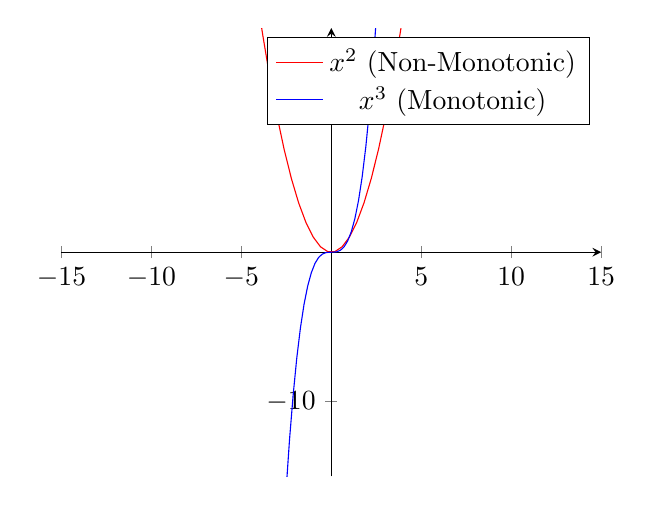
\begin{tikzpicture}
                \begin{axis}[
                    axis lines = center,
                    xmin = -15,
                    xmax = 15,
                    ymin = -15,
                    ymax = 15,
                ]
                % x^2
                \addplot [
                    domain=-20:20,
                    samples=100,
                    color=red,
                ]
                {x^2};
                \addlegendentry{$x^2$ (Non-Monotonic)}
                % x^3
                \addplot [
                    domain=-10:10,
                    samples=100,
                    color=blue,
                ]
                {x^3};
                \addlegendentry{$x^3$ (Monotonic)}
                \end{axis}
            \end{tikzpicture}
        \end{center}



    \subsection{Even and Odd Functions}
        \textbf{Even functions} $(f(-x)=f(x))$ are unchanged when reflected across the y-axis.
        \textbf{Odd functions} $(f(-x)=-f(x)$ are unchanged when rotated $180\degree$ about the origin. \\

        \begin{center}
            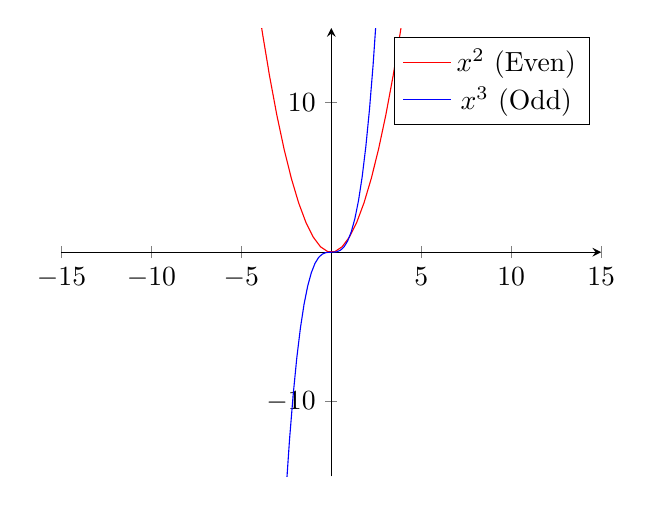
\begin{tikzpicture}
                \begin{axis}[
                    axis lines = center,
                    xmin = -15,
                    xmax = 15,
                    ymin = -15,
                    ymax = 15,
                ]
                % x^2
                \addplot [
                    domain=-20:20,
                    samples=100,
                    color=red,
                ]
                {x^2};
                \addlegendentry{$x^2$ (Even)}
                % x^3
                \addplot [
                    domain=-10:10,
                    samples=100,
                    color=blue,
                ]
                {x^3};
                \addlegendentry{$x^3$ (Odd)}
                \end{axis}
            \end{tikzpicture}
        \end{center}



    \subsection{Piecewise and Parametric Functions}
        Functions that are defined differently across its $x$-intervals are
        \textbf{piecewise functions}. Consider the function defined below \\

        \begin{equation*}
            f(x)=
            \begin{cases}
                x^2 & ,x<2 \\
                6 & ,x=2 \\
                10-x & , 2<x\leq 6
            \end{cases}
        \end{equation*}

        \noindent The domain is then $\{x\in\mathbb{R}|x\leq 6\}$ and the graph looks like this: \\

        \begin{center}
            \begin{tikzpicture} [circ/.style={circle,draw,inner sep=2pt}]
                \begin{axis}[
                    axis lines = center,
                    xmin=-4.5,
                    xmax=6.5,ymin=-2,
                    xlabel={$x$},ylabel={$y$},
                ]
                %f(x), x < 2
                \addplot [
                    red,
                    smooth,
                    {Stealth[bend]}-,
                    domain=-4:2,
                    postaction={decoration={text along path,
                    text align={align=center},
                    text={|\color{red}|{$y$}{${}={}$}{${x^2}$}},
                    raise=-2.5ex,
                    },
                    decorate}
                ]
                {x^2}
                node[pos=1,circ,fill=white]{};
                \addlegendentry{$f(x)$}
                %f(x), x = 2
                \path (2,6) node [
                    circ,
                    fill=red!60
                ]
                {};
                %f(x), 2 < x <= 6
                \addplot [
                    red,
                    samples=2,
                    domain=2:6
                ]
                {10-x};
                node[pos=0,circ,fill=white]{};
                node[pos=1,circ,fill=red!60]{};
                \end{axis}
            \end{tikzpicture}
        \end{center}

        \noindent Instead of defining a single function $y=f(x)$, \textbf{Parametric Equations} are
        defined as multiple functions together, one for each variable. Hence, we can represent a
        function with $x$ and $y$ in terms of the \textbf{parameter} $t$ as below:

        \begin{center}
            \begin{tabular} {cc}
                $x=f(t)$ & $y=g(t)$
            \end{tabular}
        \end{center}

        \noindent An example of a \textbf{parametric curve}, the set of points the parameter gives
        in all the parametric equations, is the parent circle given by $x^2+y^2=r^2$. Isolating $x$
        and $y$ give our two parametric equations, $y=\pm\sqrt{r^2-x^2}$ and $x=\pm\sqrt{r^2-y^2}$. \\

        \noindent When we sketch parametric curves, we plug in values of the parameter and find
        their x and y-values, graphing each point of the form $(x,y)$ on the Cartesian Plane.
        It is important to note that parametric curves always have a \textbf{direction of motion},
        represented by arrows on the curve given by the increasing parameter $t$.

        \noindent We can \textbf{eliminate the parameter} from a set of parametric equations by
        solving for the parameter $t$ in one of the equations and plugging the value for $t$ into
        the second parametric equation.\\

        \begin{figure} [hbt!]
            \centering
            \includegraphics [scale = 0.5] {Resources/Unit9EvenMoreFunctions/param.png}
        \end{figure}



    \subsection{The Absolute Value Function}
        An \textbf{Absolute Value Function} is a function involving absolute value operations.
        The absolute value parent function is \\

        \begin{equation*}
            f(x)=|x|=
            \begin{cases}
                x, & x>0 \\
                0, & x=0 \\
                -x, & x<0
            \end{cases}
        \end{equation*}

        \noindent Absolute value functions are V-shaped and to graph them we simply choose some
        $x$-values and plot their ordered pairs. \\

        \begin{center}
            \begin{tikzpicture}
                \begin{axis}[
                    axis lines = center,
                    xmin = -5,
                    xmax = 5,
                    ymin = -5,
                    ymax = 5
                ]
                % f(x)
                \addplot [
                    samples=100,
                    color=red,
                ]
                {abs(x)};
                \addlegendentry{$f(x)=|x|$}
                \end{axis}
            \end{tikzpicture}
        \end{center}



    \subsection{The Floor and Ceiling Functions}
        The \textbf{floor} of a number is the nearest integer down. The \textbf{ceiling} of a number
        is the nearest integer up. For 2.31, the floor is 2 and the ceiling is 3. The floor and
        ceiling of integers are the integers themselves. The floor of $x$ is represented by
        $\floor*{x}$ and the ceiling by $\ceil*{x}$. \\

        \noindent The \textbf{Floor Function} is piecewise, discontinuous at each integer, and is
        composed of the greatest integer that is less than or equal to $x$. The
        \textbf{Ceiling Function} is piecewise, discontinuous at each integer, and is composed of
        the least integer that is greater than or equal to $x$.\\

        \noindent \color{purple} \textbf{Properties of Floor and Ceiling Functions:} \color{black} \\
        1. $\floor*{x+n}=\floor*{x}+n$ for any integer $n$ \\
        2. $\floor*{x}+\floor*{-x}=\begin{cases}
                                       -1, & x \not\in \mathbb{Z}\\0, &x\in\mathbb{Z}
        \end{cases}$ \\
        3. $\floor*{x+y}=\floor*{x}+\floor*{y}=\floor*{x}+\floor*{y}+1$ \\

        \noindent Similary, all of the floor brackets can be replaced with ceiling brackets for
        their properties as well. \\

        \noindent The domain of the floor function is given by $\floor*{x}\leq x<\floor*{x}+1$. \\

        \noindent \color{blue} \textit{Example 1: Find all the values of $x$ that satisfy
        $\floor*{0.5+\floor*{x}}=20$}. \color{black} \\
        Let $y=\floor*{x}$. Then \\

        \begin{align*}
            \floor*{0.5+y} &= 20 \\
            & \iff \\
            20\leq y &+ 0.5 <21\\
            19.5\leq &y <20.5
        \end{align*}

        \noindent Since $y$ is an integer and $y=20$ is the only interval in this interval,
        this becomes $y=20=\floor*{x}$. Since any value less than 21 and greater than or equal to
        20 wil satisfy this equation, the answer is $\{x\in\mathbb{R}|20\leq x<21\}$. \\

        \begin{center}
            \begin{tikzpicture} [circ/.style={circle,draw,inner sep=1.5pt}]
                \begin{axis} [
                    axis lines = center,
                    xmin = -5,
                    xmax = 5,
                    ymin = -5,
                    ymax = 5,
                    xlabel={$x$},ylabel={$y$},
                ]
                %Floor function
                \addplot[red,samples=2,domain=-4:-3] {-4}
                    node[pos=0,circ,fill=red!60]{}
                    node[pos=1,circ,fill=white]{};
                \addplot[red,samples=2,domain=-3:-2] {-3}
                    node[pos=0,circ,fill=red!60]{}
                    node[pos=1,circ,fill=white]{};
                \addplot[red,samples=2,domain=-2:-1] {-2}
                    node[pos=0,circ,fill=red!60]{}
                    node[pos=1,circ,fill=white]{};
                \addplot[red,samples=2,domain=-1:0] {-1}
                    node[pos=0,circ,fill=red!60]{}
                    node[pos=1,circ,fill=white]{};
                \addplot[red,samples=2,domain=0:1] {0}
                    node[pos=0,circ,fill=red!60]{}
                    node[pos=1,circ,fill=white]{};
                \addplot[red,samples=2,domain=1:2] {1}
                    node[pos=0,circ,fill=red!60]{}
                    node[pos=1,circ,fill=white]{};
                \addplot[red,samples=2,domain=2:3] {2}
                    node[pos=0,circ,fill=red!60]{}
                    node[pos=1,circ,fill=white]{};
                \addplot[red,samples=2,domain=3:4] {3}
                    node[pos=0,circ,fill=red!60]{}
                    node[pos=1,circ,fill=white]{};
                \end{axis}
            \end{tikzpicture} \\
            \textbf{The Floor Function}
        \end{center}

        \begin{center}
            \begin{tikzpicture} [circ/.style={circle,draw,inner sep=1.5pt}]
                \begin{axis}[
                    axis lines = center,
                    xmin = -5,
                    xmax = 5,
                    ymin = -5,
                    ymax = 5,
                    xlabel={$x$},
                    ylabel={$y$}
                ]
                %Ceiling function
                \addplot[red,samples=2,domain=-4:-3] {-4}
                    node[pos=0,circ,fill=white]{}
                    node[pos=1,circ,fill=red!60]{};
                \addplot[red,samples=2,domain=-3:-2] {-3}
                    node[pos=0,circ,fill=white]{}
                    node[pos=1,circ,fill=red!60]{};
                \addplot[red,samples=2,domain=-2:-1] {-2}
                    node[pos=0,circ,fill=white]{}
                    node[pos=1,circ,fill=red!60]{};
                \addplot[red,samples=2,domain=-1:0] {-1}
                    node[pos=0,circ,fill=white]{}
                    node[pos=1,circ,fill=red!60]{};
                \addplot[red,samples=2,domain=0:1] {0}
                    node[pos=0,circ,fill=white]{}
                    node[pos=1,circ,fill=red!60]{};
                \addplot[red,samples=2,domain=1:2] {1}
                    node[pos=0,circ,fill=white]{}
                    node[pos=1,circ,fill=red!60]{};
                \addplot[red,samples=2,domain=2:3] {2}
                    node[pos=0,circ,fill=white]{}
                    node[pos=1,circ,fill=red!60]{};
                \addplot[red,samples=2,domain=3:4] {3}
                    node[pos=0,circ,fill=white]{}
                    node[pos=1,circ,fill=red!60]{};
                \end{axis}
            \end{tikzpicture} \\
            \textbf{The Ceiling Function}
        \end{center}



    \subsection{The Fractional Part Function}
        The \textbf{Fractional Part Function} is defined as $f(x)=\{x\}=x-\floor*{x}$.
        For nonnegative real numbers, the fractional part is simply the part after the decimal.
        For example, $\{3.64\}=3.64-\floor*{3.64}=3.64-3=0.64$. \\

        \noindent \textbf{Properties of the Fractional Part Function:} \\
        1. $0\leq\{x\}<1$ and $0=\{x\}$ if and only if $x$ is an integer \\
        2. $\{x\}+\{-x\}=$

        \begin{cases}
            0 & \text{if } x \text{ is an integer} \\
            1 & \text{otherwise}
        \end{cases}

        \noindent 3. If $a$ and $b$ are integers and $b>0$ then $\{\frac{a}{b}\}=\frac{r}{b}$, where
        $r$ is the remainder from dividing $a$ by $b$.

        \begin{center}
            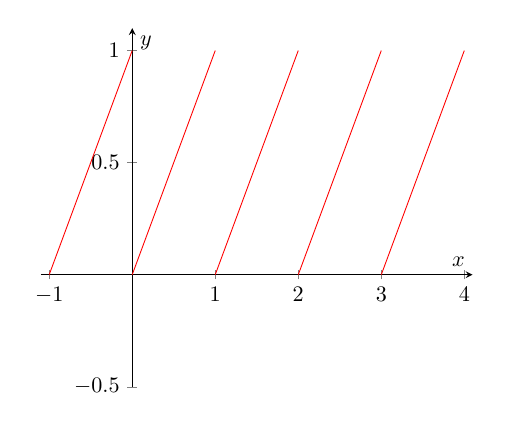
\begin{tikzpicture}[circ/.style={circle,draw,inner sep=1.5pt}, scale = 0.8]
                \begin{axis}[
                    axis lines = center,
                    xmin = -1.1,
                    xmax = 4.1,
                    ymin = -0.5,
                    ymax = 1.1,
                    xlabel={$x$},
                    ylabel={$y$}
                ]
                %Coordinates
                \coordinate (A) at (-1,0);
                \coordinate (B) at (0,1);
                \coordinate (C) at (0,0);
                \coordinate (D) at (1,1);
                \coordinate (E) at (1,0);
                \coordinate (F) at (2,1);
                \coordinate (G) at (2,0);
                \coordinate (H) at (3,1);
                \coordinate (I) at (3,0);
                \coordinate (J) at (4,1);
                %%%
                %Functions
                \draw[color=red] (A) -- (B);
                \draw[color=red] (C) -- (D);
                \draw[color=red] (E) -- (F);
                \draw[color=red] (G) -- (H);
                \draw[color=red] (I) -- (J);
                %%%
                \end{axis}
            \end{tikzpicture} \\
            \textbf{The Fractional Part Function}
        \end{center}  % Even More Functions
    \section{Conics}

    \subsection{Introduction to Conics}
        From Analytic Geometry, \textbf{Conic Sections} are the intersection of a plane and
        2 opposite-facing solid cones from different angles. \\

        \begin{figure} [hbt!]
            \centering
            \includegraphics [scale=0.6] {Resources/Unit10Conics/conics.PNG}
        \end{figure}

        \noindent These curves can be defined using a straight line (\textbf{directrix}) and a
        point (\textbf{focus}). The distance from the focus to a point on the curve and the
        distance perpendicularly from the directrix to that point will always be the same ratio.
        For ellipses, this ratio is less than 1. For parabolas, the ratio is 1, hence the
        distances are equal. For hyperbolas, this ratio is greater than 1. This ratio is called
        \textbf{eccentricity}, which graphically shows us how "un-circular" the curve is. The
        larger the eccentricity, the less curved it is. Circles have an eccentricity of 0. \\

        \begin{figure} [hbt!]
            \centering
            \includegraphics [scale=0.5] {Resources/Unit10Conics/ecc.PNG}
        \end{figure}

        \noindent The \textbf{latus rectum} runs parallel to the directrix and passes through the focus. \\
        \noindent \textbf{Length of the Latus Rectum:} \\

        \begin{center}
            \begin{tabular}{|c|c|}
                \hline
                \textbf{Parabolas} & 4x focal length  \\
                \hline
                \textbf{Circles}   & the diameter     \\
                \hline
                \textbf{Ellipses}  & $\frac{2b^2}{a}$ \\
                \hline
            \end{tabular}
        \end{center}

        \noindent Above, $a$ and $b$ are the \textbf{major} and \textbf{minor axes}, respectively.

        \begin{figure} [hbt!]
            \centering
            \includegraphics[scale = 0.6] {Resources/Unit10Conics/latrect.PNG}
            \includegraphics[scale = 0.6] {Resources/Unit10Conics/lactrect2.PNG}
        \end{figure}

        \noindent The \textbf{General Equation} that covers all conic equations is given by \\

        \begin{equation*}
            Ax^2+Bxy+Cy^2+Dx+Ey+F=0
        \end{equation*}

        \noindent where $A,B,C,D,E,F$ are all constants. \\

        \noindent \color{purple} \textbf{Process to Determine Conic Type from General Form:} \color{black} \\
        1. Are both variables squared? \\
        If no, it's a parabola. If yes, go to next step. \\
        2. Do the squared terms have opposite signs? \\
        If yes, it's a hyperbola. If no, go to next step. \\
        3. Are the squared terms multiplied by the same number? \\
        If yes, it's a circle. If no, it's an ellipse.



    \pagebreak
    \subsection{Ellipses}
        For the equations below, $a$ is the length of half of the major axis, $b$ is the length of
        half of the minor axis, and $A,C,D,E,F$ are constants, respectively. \\

        \begin{center}
            \begin{tabular}{|c|c|}
                \hline
                \textbf{General Form}
                & $Ax^2+Cy^2+Dx+Ey+F=0$                       \\
                \hline
                \textbf{Standard Form, Horizontal Major Axis}
                & $\frac{(x-h)^2}{a^2}+\frac{(y-k)^2}{b^2}=1$ \\
                \hline
                \textbf{Standard Form, Vertical Major Axis}
                & $\frac{(x-h)^2}{b^2}+\frac{(y-k)^2}{a^2}=1$ \\
                \hline
            \end{tabular}
        \end{center}

        \noindent Center: $(h,k)$ \\
        Length of Major Axis: $2a$ \\
        Length of Minor Axis: $2b$ \\
        Distance between center and foci, represented by $c$, is $c^2=a^2-b^2,a>b>0$ \\

        \noindent The major axis runs between the vertices, whereas the minor axis runs between
        the co-vertices. \\

        \begin{figure} [hbt!]
            \centering
            \includegraphics [scale=0.6] {Resources/Unit10Conics/ellipse1.jpg}
        \end{figure}

        \noindent \color{purple} \textbf{Graphing Ellipses:} \color{black} \\
        Determine the major axis, vertices, co-vertices, and foci. \\
        \textbf{Equation is in form $\frac{(x-h)^2}{a^2}+\frac{(y-k)^2}{b^2}=1, a>b$}

        \begin{center}
            \begin{tabular} {|c|c|}
                \hline
                Center                         & $(h,k)$              \\
                \hline
                Major Axis                     & parallel to $x$-axis \\
                \hline
                Coordinates of the Vertices    & $(h\pm a, k)$        \\
                \hline
                Coordinates of the Co-vertices & $(h,k \pm b)$        \\
                \hline
                Coordinates of the Foci        & $(h\pm c, k)$        \\
                \hline
            \end{tabular}
        \end{center}

        \noindent \textbf{Equation is in form $\frac{(x-h)^2}{b^2}+\frac{(y-k)^2}{a^2}=1, a>b$} \\

        \begin{center}
            \begin{tabular} {|c|c|}
                \hline
                Center                         & $(h,k)$              \\
                \hline
                Major Axis                     & parallel to $y$-axis \\
                \hline
                Coordinates of the Vertices    & $(h, k\pm a)$        \\
                \hline
                Coordinates of the Co-vertices & $(h\pm b, k)$        \\
                \hline
                Coordinates of the Foci        & $(h, k\pm c)$        \\
                \hline
            \end{tabular}
        \end{center}

        \noindent \color{blue} \textit{Example 1: Graph $\frac{(x+2)^2}{4}+\frac{(y-5)^2}{9}=1$}
        \color{black} \\
        \noindent Because $a$ is the always the bigger number, $a^2=9$ and $b^2=4$. Because
        $9>4$ the major axis is parallel to the $y$-axis. The center $(h,k)$ is then $(-2,5)$. The
        vertices are $(h,k\pm a)=(-2,2),(-2,8)$. The co-vertices are $(h\pm b,k)=(-4,5),(0,5)$.
        Since $c^2=a^2-b^2=9-4=5\implies c=\pm\sqrt{5}$, the foci are $(h,k\pm c)=(-2,5-\sqrt{5}),
        (-2,5\pm 5)$. \\

        \begin{figure} [hbt!]
            \centering
            \includegraphics [scale=0.5] {Resources/Unit10Conics/ellipse2.PNG}
        \end{figure}

        \noindent \color{blue} \textit{Example 2: Graph the ellipse given by
        $4x^2+9y^2-40x+36y+100=0$} \color{black}  \\

        \begin{align*}
            (4x^2-40x)+(9y^2+36y) &= -100 \\
            4(x^2-10x) + 9(y^2+4y) &= -100 \\
            4(x^2-10x+25)+9(y^2+4y+4) &= -100 + 100 +36 \\
            4(x-5)^2+9(y+2)^2 &= 36 \\
            \frac{(x-5)^2}{9}+\frac{(y+2)^2}{4}=1
        \end{align*}

        \noindent Because $9>4$. the major axis is parallel to the $x$-axis. Since $a^2=9$ and
        $b^2=4$, $c^2=9-4\implies c=\pm \sqrt{5}$. The center is $(5, -2)$. The vertices are
        $(2,-2),(8,-2)$. The co-vertices are $(5,-4),(5,0)$. The foci are $(5-\sqrt{5},-2),
        (5+\sqrt{5},-2)$. \\

        \begin{figure} [hbt!]
            \centering
            \includegraphics [scale=0.5] {Resources/Unit10Conics/ellipse3.PNG}
        \end{figure}



    \subsection{Circles}
        A \textbf{circle} is the set of all points on a plane that are a fixed distance from the
        center. A circle is not a function because it fails the vertical line test. A circle is a
        special type of ellipse with equations below. \\

        \begin{center}
            \begin{tabular} {|c|c|}
                \hline
                \textbf{General Form}
                & $x^2+y^2+Cx+Dy+E=0$   \\
                \hline
                \textbf{Standard Form}
                & $(x-h)^2+(y-k)^2=r^2$ \\
                \hline
            \end{tabular}
        \end{center}

        \noindent Above, the center is given by $(h,k)$ and the radius as $r$.

        \noindent \color{purple} \textbf{Graphing Circles:} \color{black} \\
        Determine the center $(h,k)$ and radius $r$ and graph it.



    \subsection{Parabolas}
        We have already graphed and worked with parabolas in the past, so here are the general
        forms of parabolas when used in the context of conics. \\

        \begin{center}
            \begin{tabular} {|c|c|c|}
                \hline
                \textbf{Parabola, Horizontal Axis}
                & $(y-k)^2=4p(x-h),p\not=0$
                & Vertex is $(h,k)$ \\
                & & Focus is $(h+p,k)$            \\
                & & Directrix is the line $x=h-p$ \\
                & & Axis is the line $y=k$        \\
                \hline
                \textbf{Parabola, Vertical Axis}
                & $(x-h)^2=4p(y-k),p\not=0$
                & Vertex is $(h,k)$ \\
                & & Focus is $(h,k+p)$            \\
                & & Directrix is the line $y=k-p$ \\
                & & Axis is the line $x=h$        \\
                \hline
            \end{tabular}
        \end{center}



    \subsection{Hyperbolas}
        Hyperbolas look like this: \\
        \begin{figure} [hbt!]
            \centering
            \includegraphics [scale=0.3] {Resources/Unit10Conics/hyperbola.png}
        \end{figure}

        \begin{center}
            \begin{tabular} {|c|c|}
                \hline
                \textbf{General Form}
                & $Ax^2-Cy^2+Dx+Ey+F=0$                       \\
                \hline
                \textbf{Hyperbola, Horizontal Transverse Axis}
                & $\frac{(x-h)^2}{a^2}-\frac{(y-k)^2}{b^2}=1$ \\
                \hline
                \textbf{Hyperbola, Vertical Transverse Axis}
                & $\frac{(y-k)^2}{a^2}-\frac{(x-h)^2}{b^2}=1$ \\
                \hline
            \end{tabular}
        \end{center}

        \noindent Center: $(h,k)$ \\
        Distance between vertices: $2a$ \\
        Distance between foci: $2c$ \\
        $c^2=a^2+b^2$ \\

        \noindent The eccentricity, $e$, has the formula \\
        $e=\frac{\sqrt{a^2+b^2}}{a}$  \\

        \noindent The reciprocal function $f(x)=\frac{1}{x}$ is a hyperbola. % Conics
    \section{Sequences and Series}

    \subsection{Introduction to Sequences and Series}
        A \textbf{sequence} is an ordered list of numbers, whereas a \textbf{series} is the
        sum of the terms of a sequence. We can represent a series with $\{a_n\}^\infty_{n=1}$,
        where the sequence starts with index $n=1$ and runs to infinity. The other notation,
        summation notation, is written $\sum^{10}_{n=1}a_n$, where the sequence runs from $n=1$
        to infinity. \\

        \noindent For example, the expansion of
        $\{a_n\}_{n=1}^{n=10}$ is $a_n=n^2=1,4,,9,16,25,36,49,64,81,100$. \\

        \noindent Conventionally, the following symbols are used:

        \begin{center}
            \begin{tabular} {|c|c|}
                \hline
                $a$
                & first term in sequence                                                    \\
                \hline
                $n$
                & number of terms in sequence                                               \\
                \hline
                $S_n$
                & sum of first $n$ terms in sequence                                        \\
                \hline
                $d$
                & Common difference between any two consecutive terms, arithmetic sequences \\
                \hline
                $r$
                & Common ratio between two consecutive terms, geometric sequences           \\
                \hline
            \end{tabular}
        \end{center}



    \subsection{Arithmetic Progressions} \\
        \textbf{Arithmetic Progressions} are sequences containing numbers which differ from each
        other by a common difference, $d$. \\

        \noindent \textbf{Formula for Arithmetic Sequences} \\

        \begin{equation*}
            a_n=a_1+d(n-1)
        \end{equation*}

        \noindent $a_n$ is the $n^{th}$ term, $a_1$ is the first term, $n$ is the index \\

        \noindent  The sum of the first $n$ terms is given by one of the three formulas. \\

        \begin{align*}
            S_n=\frac{n}{2}[2a+d(n-1)] \\
            S_n=\frac{n}{2}[a+a_n] \\
            S_n=n\cdot (middle term)
        \end{align*}

        \noindent Find the sum of the first 50 odd positive integers. \\

        \begin{equation*}
            S_n=\frac{n}{2}(2a+d(n-1))
            \implies
            S_{50}=25\cdot (2+49\cdot 2)=2500
        \end{equation*}



    \subsection{Geometric Sequences and Series}
        \textbf{Geometric Sequences} include terms that are multiplied by a ratio iteratively.
        They are given by the following formula. \\

        \begin{equation*}
            a_n=a\cdot r^{n-1}
        \end{equation*}

        \noindent $a_n$ is the $n^{th}$ term, $a$ is the first term, $r$ is the common ratio. \\

        \noindent The sum of a geometric sequence is given by \\

        \begin{equation*}
            S_n = \begin{cases}
                      a\cdot (\frac{r^n-1}{r-1}), & r\not=1 \\
                      a\cdot n, & r=1
            \end{cases}
        \end{equation*}

        \noindent The sum to infinity of a geometric sequence, where $|r|<1$, is given by \\

        \begin{equation*}
            S_\infty=\frac{a}{1-r}
        \end{equation*}

        \noindent \color{blue} \textit{Example: After striking the floor, a tennis ball bounces
        to $\frac{2}{3}$ of the height from which it last fell. What is the total vertical
        distance it travels before it comes to rest when it is dropped from a vertical height of
        100$m$?} \color{black} \\

        \noindent If $h$ is the height in meters, $e$ is a number such that $0<e<1$, and $S$ is
        the total vertical distance covered before coming to rest, then \\

        \begin{align*}
            S &= h+2(eh)+2(e^2h)+2(e^3h)+2(e^4)h + \dots \\
            &= h+2eh(1+e+e^2+e^3+\dots) \\
            &= h+2eh \cdots \frac{1}{1-e}, \because e<1 \\
            &= h\left(\frac{1+e}{1-e}\right)
        \end{align*}

        \noindent Since it is given that $h=100$ and $e=\frac{2}{3}$, \\

        \begin{equation*}
            S=100\left(\frac{1+\frac{2}{3}}{1-\frac{2}{3}}\right)=500 \text{ meters}
        \end{equation*}



    \subsection{Binomial Expansion}
        The \textbf{Binomial Theorem} allows us to expand binomials such that \\

        \begin{equation*}
            (a+b)^n
            = \sum^n_{k=0}\binom{n}{k}a^{n-k}b^k
        \end{equation*}

        \noindent where $\binom{n}{k}$, pronounced "n choose k" because it describes how many
        ways to choose $k$ elements from a set of $n$, is given by the formula \\

        \begin{equation*}
            \binom{n}{k}=\frac{n!}{k!(n-k)!}
        \end{equation*}

        \noindent In the Binomial Theorem, $\binom{n}{k}$ determines the coefficients of the
        expanded binomial. Coefficients of Binomials follow Pascal's Triangle and they match up
        like so: \\

        \begin{figure} [hbt!]
            \centering
            \includegraphics[scale = 0.5] {Resources/Unit11Sequences/pascal.PNG}
        \end{figure}

        \noindent \color{blue} \textit{Example 1: Expand $(y+5)^4$} \color{black} \\

        \begin{align*}
            (y+5)^4 &= \binom{4}{0}y^45^0
            + \binom{4}{1}y^35^1
            + \binom{4}{2}y^25^2
            + \binom{4}{3}y^15^3
            + \binom{4}{4}y^05^4 \\
            &= y^4+20y^3+150y^2+500y+625
        \end{align*}

        \noindent \color{blue} \textit{Example 2: What is the coefficient of $x^3 in (2x+4)^8?$}
        \color{black} \\
        The term containing $x^3$ is \\

        \begin{align}
            \binom{8}{5}(2x)^34^5 &= 56(2x^3)(4^5) \\
            &= 458752x^3
        \end{align}

        \noindent Hence, the coefficient is 458752. % Sequences and Series
    \section{The Cauchy-Schwartz Inequality}

    The Cauchy-Schwartz Inequality, or the Cauchy-Bunyakovsky-Schwartz Inequality, states
    that for all sequences of real numbers $a_i$ and $b_i$, we have \\

    \begin{equation*}
        (\sum^n_{i=1}a_i^2)
        (\sum^n_{i=1}b_i^2)
        \geq
        (\sum^n_{i=1}a_ib_i)^2
    \end{equation*}

    \noindent Equality holds if and only if $a_i=kb_i$ for some non-zero constant
    $k\in\mathbb{R}$. \\

    \noindent \color{blue} \textit{Example: If $x^2+y^2+z^2=1$, what is the maximum
    value of $x+2y+3z$?} \color{black} \\

    \noindent We have $(x+2y+3z)^2\leq(1^2+2^2+3^2)(x^2+y^2+z^2)=14$. Hence, $x+2y+3z\leq\sqrt{14}$
    with equality holding when $\frac{x}{1}=\frac{y}{2}=\frac{z}{3}$. Together with
    $x^2+y^2+z^2=1$, we get \\

    \begin{equation*}
        x=\frac{1}{\sqrt{14}},
        y=\frac{2}{\sqrt{14}},
        z=\frac{3}{\sqrt{14}}
    \end{equation*} % The Cauchy-Schwartz Inequality
    \section{Symbolic Logic and Proofs}

    \subsection{Statements and Logical Operators}
        A \textbf{proof} is an argument from \textbf{hypotheses} to a \textbf{conclusion}.
        Proofs usually begin with \textbf{premises}, statements that are known to be true.
        The \textbf{Rule of Premises} says that you may write down a premise at any point in a
        proof. The rule of \textbf{modus ponendo ponens} says that if you know $P$ and
        $P\rightarrow Q$, you can write down $Q$. \\

        \noindent Mathematical statements can only be true or false. The letters $p$ and $q$
        often denote statements. \\

        \noindent \color{purple} \textbf{Logical Operators:} \color{black} \\
        \textbf{Not ($\neg$)}: The statement "not $p$" is called the \textbf{negation} of $p$. \\

        \begin{center}
            \begin{tabular} {|c|c|}
                \hline
                $p$ & $\neg p$ \\
                \hline
                0   & 1        \\
                \hline
                1   & 0        \\
                \hline
            \end{tabular}
        \end{center}

        \noindent \textbf{Double Negation} states that $\neg\neg P$ is logically equivalent to $P$.

        \noindent \textbf{And (\&)}: \\

        \begin{center}
            \begin{tabular} {|c|c|c|}
                \hline
                $p$ & $q$ & $p\& q$ \\
                \hline
                1 & 1 & 1 \\
                \hline
                1 & 0 & 0 \\
                \hline
                0 & 1 & 0 \\
                \hline
                0 & 0 & 0 \\
                \hline
            \end{tabular}
        \end{center}

        \noindent \textbf{Or: ($\vert\vert$)} \\

        \begin{center}
            \begin{tabular} {|c|c|c|}
                \hline
                $p$ & $q$ & $p||q$ \\
                \hline
                1   & 1   & 1      \\
                \hline
                1   & 0   & 1      \\
                \hline
                0   & 1   & 1      \\
                \hline
                0   & 0   & 0      \\
                \hline
            \end{tabular}
        \end{center}

        \noindent\textbf{If\dots then ($\rightarrow)$:} \\

        \begin{center}
            \begin{tabular} {|c|c|c|}
                \hline
                $p$ & $q$ & $p\rightarrow q$ \\
                \hline
                1   & 1   & 1                \\
                \hline
                1   & 0   & 0                \\
                \hline
                0   & 1   & 1                \\
                \hline
                0   & 0   & 1                \\
                \hline
            \end{tabular}
        \end{center}

        \noindent If $p$ is false then $p\rightarrow q$ is \textbf{vacuously true}.
        For example, the statement all cell phones in the room are turned off is true even
        if there are no cell phones in the room. \\

        \noindent \textbf{If and only if ($\iff$):} \\

        \begin{center}
            \begin{tabular} {|c|c|c|}
                \hline
                1 & 1 & 1 \\
                \hline
                1 & 0 & 0 \\
                \hline
                0 & 1 & 0 \\
                \hline
                0 & 0 & 1 \\
                \hline
            \end{tabular}
        \end{center}

        \noindent When $p\iff q$ is true, $p$ and $q$ are \textbf{equivalent}. \\

        \noindent \textbf{Quantifiers} include the phrases "for every ($\forall$)" and
        "there exists (\exists)". $Consider the sentence "$x$ is even". This does not count
        as a statement since we can't say whether or not it is true or false since we don't
        know what $x$ is. We can make this a statement by saying "an integer $x$ is even if
        there exists an integer $y$ such that $x=2y$".$



    \subsection{Proof Methods}
        \noindent \color{purple} \textbf{Proof by Cases:} \color{black} \\
        \color{blue} \textit{Example: For every integer $x$, the integer $x(x+1)$ is even.} \color{black}  \\
        Let $x$ be any integer. Then $x$ is even or odd. \\
        Case 1: suppose $x$ is even. Choose an integer $k$ such that $x=2k$. Then $x(x+1)=2k(2k+1)$.
        Let $y=k(2k+1)$; then $y$ is an integer and $x(x+1)=2y$ so $x(x+1)$ is even. \\
        Case 2: suppose $x$ is odd. Choose an integer $k$ such that $x=2k+1$. Then
        $x(x+1)=(2k+1)(2k+2)$. Let $y=(2k+1)(k+1)$; then $x(x+1)=2y$, so $x(x+1)$ is even.
        $\blacksquare$ \\

        \noindent \color{purple} \textbf{Proof by Contradiction:} \color{black} \\
        Suppose we want to prove that statement $p$ is true. We begin by assuming $p$ is false.
        We then deduce a \textbf{contradiction} (some statement about $q$ we know to be false).
        If we succeed, then our assumption that $p$ is false must be wrong. Hence $p$ would have
        to be true. % Symbolic Logic and Proofs

\end{document}